\documentclass{if-beamer}
\usepackage{listings}
\usepackage{svg}
\usepackage{graphicx}
\usepackage{xcolor}
\usepackage{wrapfig}


\definecolor{keywords1}{RGB}{193,89,45}
\definecolor{keywords2}{RGB}{55,80,146}
\definecolor{string}{RGB}{57,181,45}


\lstdefinelanguage{Cypher}{
	keywords={MATCH, WHERE, RETURN, CREATE, SET, DELETE, WITH, UNWIND, OPTIONAL, FOREACH, MERGE, ORDER, BY, ASC, DESC, DISTINCT, LIMIT, SKIP},
	keywordstyle=\color{blue}\bfseries,
	ndkeywords={NODE, RELATIONSHIP, PROPERTIES},
	ndkeywordstyle=\color{purple}\bfseries,
	sensitive=true,
	comment=[l]{//},
	morecomment=[s]{/*}{*/},
	commentstyle=\color{gray}\ttfamily,
	stringstyle=\color{red}\ttfamily,
	morestring=[b]',
	morestring=[b]"
}


\lstdefinelanguage{pseudocodigo}{
	keywords=[1]{Inicializa, Enquanto, Algoritmo, Faca, Se, Entao, Senao, Para, Cada, Retire,Ponha, Numere},
	keywords=[2]{Saida, Entrada},
	keywordstyle=[1]\color{keywords1}\bfseries,
	keywordstyle=[2]\color{keywords2}\bfseries,
	commentstyle=\itshape,
	string=[b]{"},
	stringstyle=\color{string},
	breaklines=true,
	breakatwhitespace=true,
	tabsize=4
}

% --------------------------------------------------- %
%                  Presentation info	              %
% --------------------------------------------------- %
\title[PCO001]{PCO001\\ALGORITMOS E ESTRUTURAS DE DADOS}
\subtitle{Seminário - Grafos}
\author{Carlos Henrique Reis}
\institute[UNIFEI]{
  Universidade Federal de Itajubá - UNIFEI
}
\date{\today}
%\logo{
%\includegraphics[scale=0.25]{simbolo300x300.png}
%}

\subject{} % metadata

\graphicspath{{figuras/}}
% --------------------------------------------------- %
%                    Title + Schedule                 %
% --------------------------------------------------- %

\begin{document}

\begin{frame}
  \titlepage
\end{frame}

\begin{frame}{Sumário}
  \tableofcontents
\end{frame}

% --------------------------------------------------- %
%                      Presentation                   %
% --------------------------------------------------- %

\section{Considerações Iniciais}

\begin{frame}{Considerações Iniciais}
\begin{itemize}
\justifying
\item Em diversas aplicações computacionais, surge a necessidade de \textbf{modelar}, representar e analisar algum conjunto de conexões entre pares de objetos.\pause

\item Para lidar com essas questões, a Ciência da Computação oferece uma estrutura fundamental: o grafo. Grafos são abstrações matemáticas que modelam conjuntos de objetos (vértices) e suas conexões (arestas), permitindo representar e analisar relacionamentos complexos de forma eficiente.

\begin{figure}
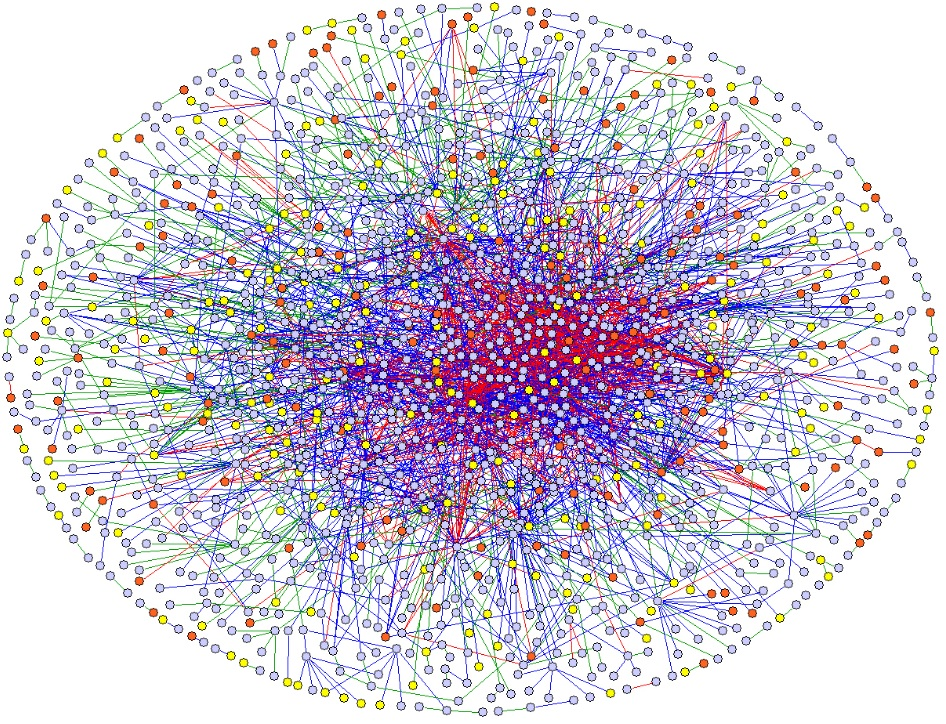
\includegraphics[scale=0.2]{Figuras/slide-1.jpg} 
\caption{Exemplo modelagem em grafos  }
\end{figure}

\end{itemize} 
\end{frame}

\begin{frame}{Considerações Iniciais}

\justifying
Como o Google Maps consegue calcular qual é a menor distância entre a minha casa e o supermercado?

\begin{figure}
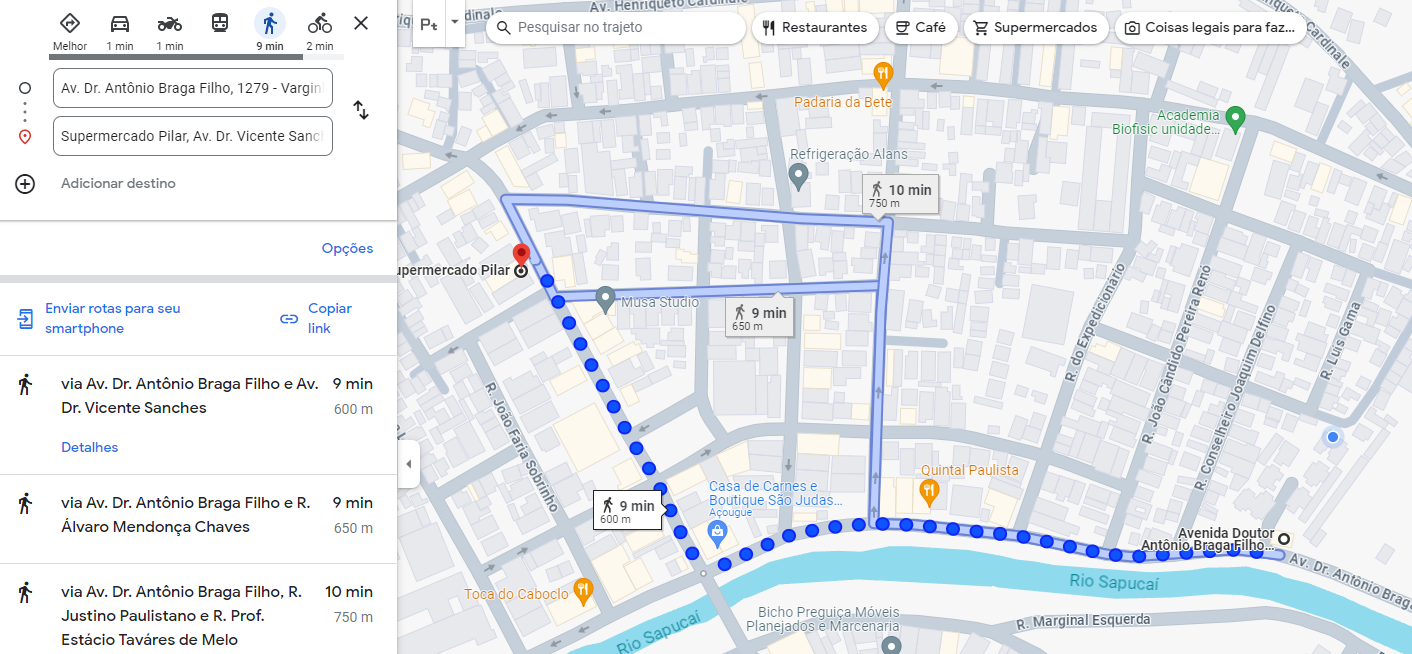
\includegraphics[scale=0.3]{Figuras/exemplos-grafo/a.png} 
\caption{Exemplo caminho ideal entre dois pontos}
\end{figure} 
\end{frame}

\begin{frame}{Considerações Iniciais}
\begin{itemize}
\justifying
\item Uma das formas seria modelar a rede de ruas, levando em conta distância, direção ou o tempo estimado para percorrer aquele trecho, ou seja, podemos tratar as esquinas como nossos objetos e as ruas como conjunto de conexões.
\item Assim o aplicativo pode utilizar algoritmos poderosos para encontrar o caminho com o menor peso total, ou seja, o trajeto mais eficiente entre a minha casa e o supermercado.
\begin{figure}
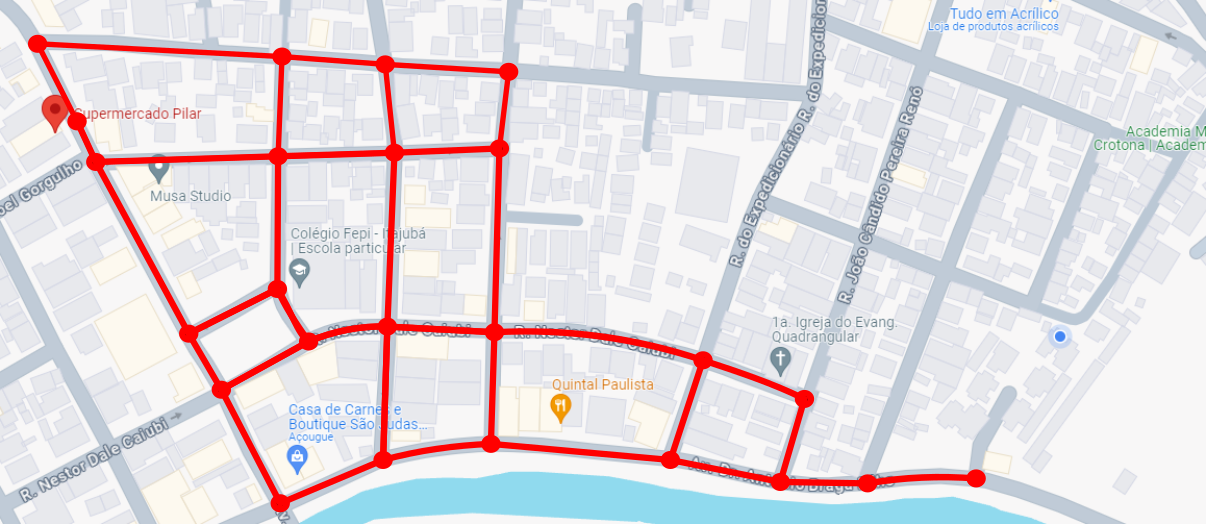
\includegraphics[scale=0.33]{Figuras/exemplos-grafo/b.png} 
\caption{Exemplo da modelagem de um grafo}
\end{figure}
\end{itemize} 
\end{frame}

\section{Definições}

\begin{frame}{Definições} 
\begin{itemize}
\justifying
\item Praticamente qualquer objeto pode ser representado como um grafo.
\item Um grafo $G(V,A)$ é definido por dois conjuntos 
\begin{itemize}
\vspace{0.3cm}
\item Conjunto V de vértices (não vazio): Objetos simples que podem ter nome e outros atributos.
\vspace{0.3cm}
\item Conjunto A de arestas: Utilizadas para conectar pares de vértices.
\end{itemize} 
\begin{figure}
  \centering
  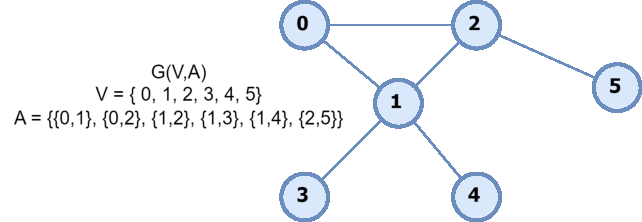
\includegraphics[scale=0.80]{Figuras/exemplos-grafo/e_svg-tex.pdf}
  \caption{Representação matemática de um grafo}
\end{figure}

\end{itemize} 
\end{frame}

\begin{frame}{Definições} 
\begin{itemize}
\justifying
\item \textbf{Vértice} é cada um dos itens representados no grafo.
\begin{itemize}
\vspace{0.3cm}
\item O seu significado depende da natureza do problema modelado como: Pessoas, uma tarefa em um projeto, lugares em um mapa, etc.
\end{itemize}
\item \textbf{Aresta (ou arco)} liga dois vértices e diz qual a relação entre eles
\begin{itemize}
\vspace{0.3cm}
\item Dois vértices são  \textbf{adjacentes} se existir uma aresta ligando eles: Pessoas (parentesco entre elas ou amizade), tarefas de um projeto (pré-requisito entre as tarefas), lugares de um mapa (estradas que existem ligando os lugares), etc
\end{itemize} 
\begin{figure}
  \centering
  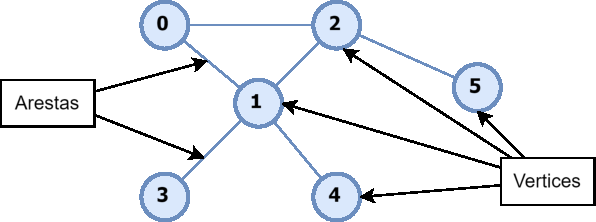
\includegraphics[scale=0.80]{Figuras/exemplos-grafo/f_svg-tex.pdf}
  \caption{Vértices e arestas de um grafo}
\end{figure}

\end{itemize} 
\end{frame}

\begin{frame}{Tipos de arestas} 
\begin{itemize}
\justifying
\item \textbf{Direcionadas}: A conexão tem uma direção específica, indicando um fluxo ou relação assimétrica.
\item \textbf{Não direcionadas}: A conexão não tem direção, representando uma relação simétrica.
\item \textbf{Ponderadas}: As arestas possuem um valor numérico (peso) associado, que pode representar custo, distância, capacidade, etc.
\begin{figure}
  \centering
  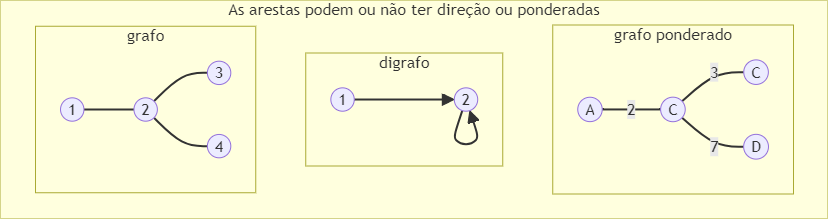
\includegraphics[scale=0.35]{Figuras/exemplos-grafo/i.png}
  \caption{Exemplos de arestas}
\end{figure}

\end{itemize} 
\end{frame}

\begin{frame}{Grau de um Vértice} 
\begin{itemize}
\justifying
\item Em grafos não direcionados
\begin{itemize}
\vspace{0.3cm}
\item O grau de um vértice indica quantas arestas estão conectadas a ele. Em outras palavras, é o número de vizinhos que o vértice possui.
\end{itemize}
\item Grau em Dígrafos (Grafos Direcionados):
\begin{itemize}
\vspace{0.3cm}
\item O grau de um vértice é o número de arestas que saem dele (out-degree) mais o número de arestas que chegam nele (in-degree).
\end{itemize}
\begin{figure}
  \centering
  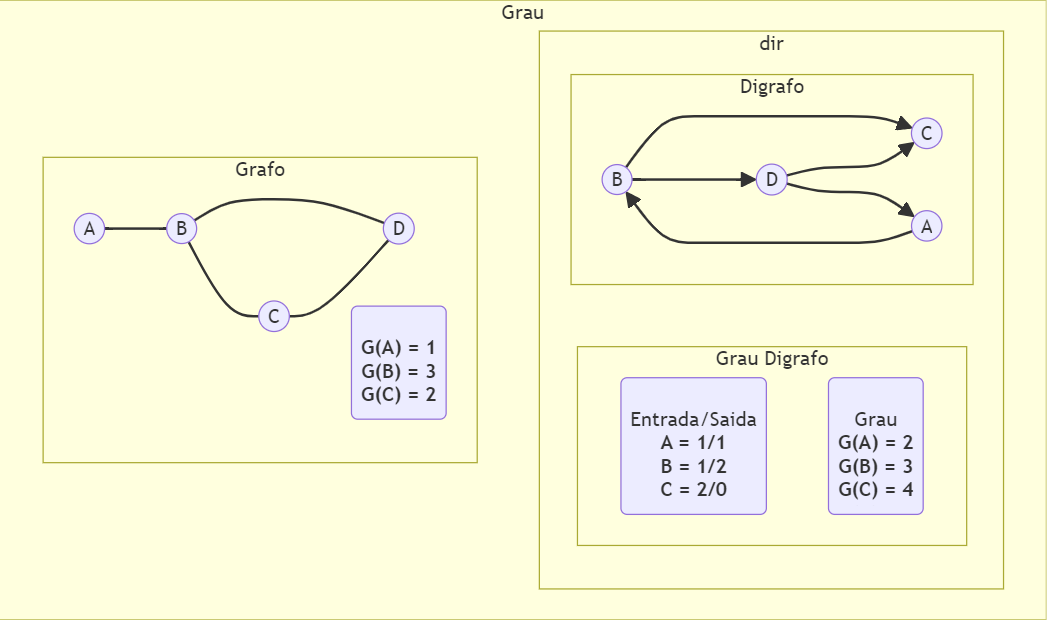
\includegraphics[scale=0.20]{Figuras/exemplos-grafo/h.png}
\end{figure}

\end{itemize} 
\end{frame}

\begin{frame}{Ciclos, caminhos e laços} 
\begin{itemize}
\justifying
\item Um laço é uma aresta que conecta um vértice a ele mesmo. Laços podem representar auto referências ou loops em um sistema

\item Um caminho é uma sequência de vértices conectados por arestas. Em um caminho válido, cada vértice é adjacente ao próximo vértice na sequência.

\item O comprimento de um caminho é definido pelo número de arestas que o compõem (ou, equivalentemente, o número de vértices menos 1).

\item Um ciclo é um caminho que começa e termina no mesmo vértice. Ou seja, é um caminho fechado.

\item OBS: A principal diferença entre um caminho e um ciclo é que um caminho tem pontos inicial e final distintos, enquanto um ciclo começa e termina no mesmo vértice.

\begin{figure}
  \centering
  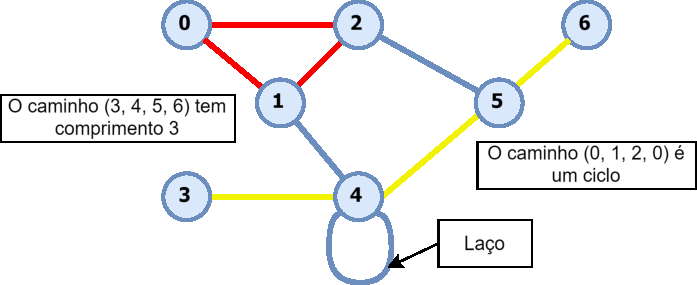
\includegraphics[scale=0.80]{Figuras/exemplos-grafo/k_svg-tex.pdf}
\end{figure}

\end{itemize} 
\end{frame}

\section{Tipos de Grafos}

\begin{frame}{Tipos de Grafos} 

\justifying
Grafo trivial
\begin{itemize}
\item  Possui um único vértice e nenhuma aresta
\end{itemize} 
Grafo simples 
\begin{itemize}
\item  Grafo não direcionado, sem laços e sem arestas paralelas (multigrafo)
\end{itemize} 
Grafo completo 
\begin{itemize}
\item  Grafo simples onde cada vértice se conecta a todos os outros vértices do grafo.
\end{itemize} 
Grafo regular
\begin{itemize}
\item  Grafo onde todos os seus vértices possuem o mesmo grau (número de arestas ligadas a ele) 
\end{itemize} 

Todo grafo completo é também regular

\begin{figure}[h]
\centering
\begin{minipage}[b]{0.45\textwidth}
  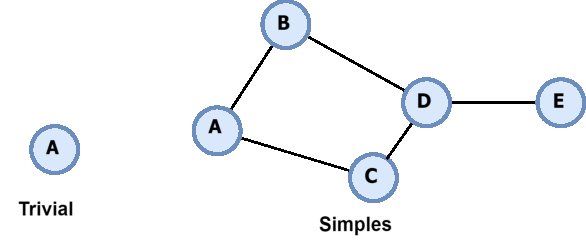
\includegraphics[width=\textwidth]{Figuras/exemplos-grafo/l_svg-tex.pdf}
  \label{fig:imagem2}
\end{minipage}
\hfill
\begin{minipage}[b]{0.45\textwidth}
  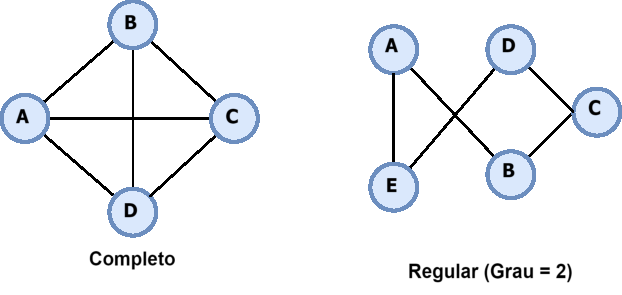
\includegraphics[width=\textwidth]{Figuras/exemplos-grafo/m_svg-tex.pdf}
  \label{fig:imagem3}
\end{minipage}
\end{figure}
\end{frame}

\begin{frame}{Tipos de Grafos} 

\justifying
Subgrafo
\begin{itemize}
\item  Um grafo menor contido dentro de um grafo maior. Usado para analisar partes específicas de um grafo.
\end{itemize} 
Grafo conexo e desconexo 
\begin{itemize}
\item  Grafo conexo: existe um caminho ligando quaisquer dois vértices.
\item  Quando isso não acontece, temos um grafo desconexo
\end{itemize} 

\begin{figure}[h]
\centering

  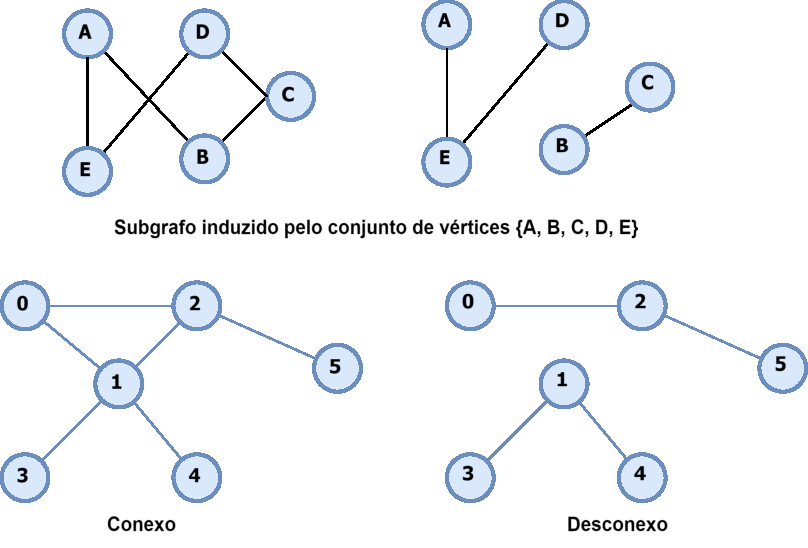
\includegraphics[scale=0.50]{Figuras/exemplos-grafo/n_svg-tex.pdf}
  
  \label{fig:imagem4}
\end{figure}
\end{frame}

\begin{frame}{Tipos de Grafos} 

\justifying
Grafo bipartido
\begin{itemize}
\item  Vértices divididos em dois conjuntos, com arestas conectando apenas vértices de conjuntos diferentes. Modela relações entre dois tipos de entidades.
\end{itemize} 
Grafos isomorfos
\begin{itemize}
\item  Mesma estrutura, mas com diferentes rótulos nos vértices e arestas. Essencialmente, o mesmo grafo rearranjado e "renomeado".
\end{itemize} 
Grafos Ponderados
\begin{itemize}
\item  Arestas possuem pesos numéricos, representando custos, distâncias ou outras métricas.
\end{itemize} 

\begin{figure}[h]
\centering

  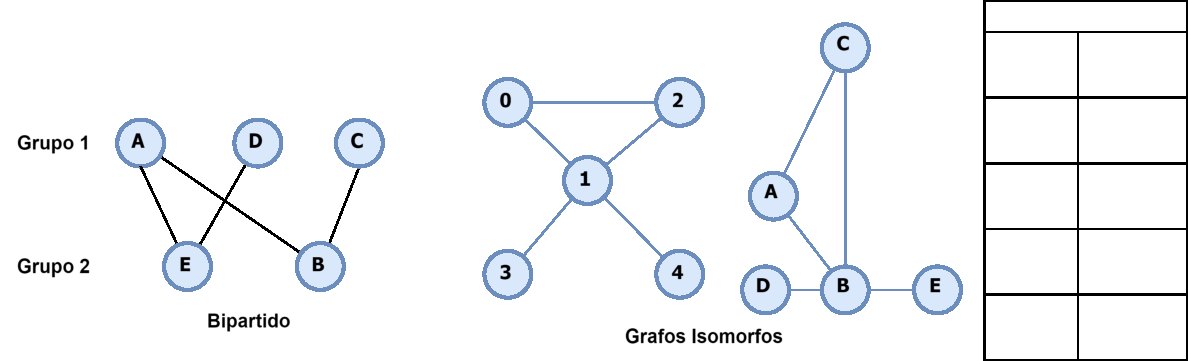
\includegraphics[scale=0.50]{Figuras/exemplos-grafo/o_svg-tex.pdf}
  
  \label{fig:imagem5}
\end{figure}
\end{frame}


\begin{frame}{Tipos de Grafos} 

\justifying
Grafo Euleriano
\begin{itemize}
\item  Possui um ciclo que visita todas as arestas exatamente uma vez. Útil para problemas de roteamento.
\end{itemize} 
Grafo Semi-Euleriano
\begin{itemize}
\item  Possui um caminho (não necessariamente um ciclo) que visita todas as arestas exatamente uma vez.
\end{itemize} 
Grafo Hamiltoniano
\begin{itemize}
\item  Possui um caminho que visita todos os vértices exatamente uma vez.
\end{itemize} 

\begin{figure}[h]
\centering

  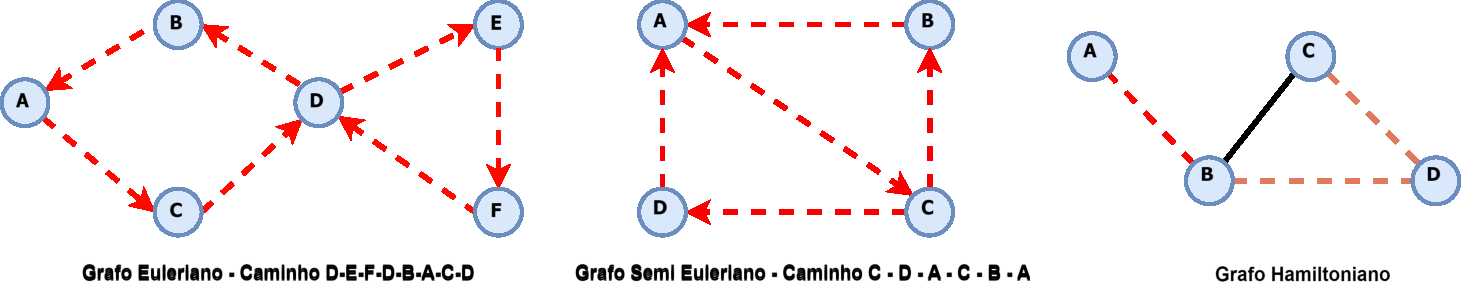
\includegraphics[scale=0.40]{Figuras/exemplos-grafo/p_svg-tex.pdf}
  
  \label{fig:imagem1}
\end{figure}
\end{frame}


\section{Representação}

\begin{frame}{Representação} 

\justifying
Existem diferentes maneiras de representar um grafo, as mais comuns são a \textbf{Matriz de adjacência} e \textbf{Lista de adjacência}.\pause

\textbf{Matriz de adjacência}
\begin{itemize}
\item  Estrutura: Matriz $NxN$ (N = número de vértices).
\item  Arestas: Representadas por marcas na posição $(i, j)$ da matriz, indicando conexão entre vértices $i$ e $j$.
\item  Custo Computacional: $O(N^2)$ - alto custo, especialmente para grafos com muitos vértices.
\end{itemize} 

\begin{figure}
  \centering
  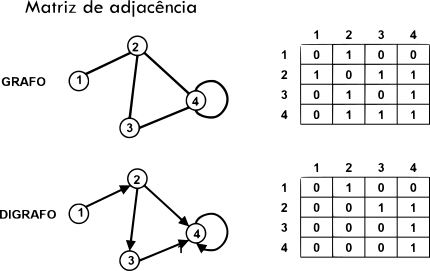
\includegraphics[scale=0.70]{Figuras/exemplos-grafo/q.png}
\end{figure}
\end{frame}


\begin{frame}{Representação} 
	
	\justifying
	Existem diferentes maneiras de representar um grafo, as mais comuns são a \textbf{Matriz de adjacência} e \textbf{Lista de adjacência}.\pause
	
	\textbf{Lista de adjacência}
	

	\begin{itemize}
		\item  Estrutura: Cada vértice possui uma lista contendo seus vértices adjacentes (vizinhos).
		\item  Arestas: Representadas pela presença de um vértice na lista de outro.
		\item  Custo Computacional: $O(V+E)$ - mais eficiente para grafos esparsos (V = vértices, E = arestas).
	\end{itemize} 
	
	\begin{figure}
		\centering
		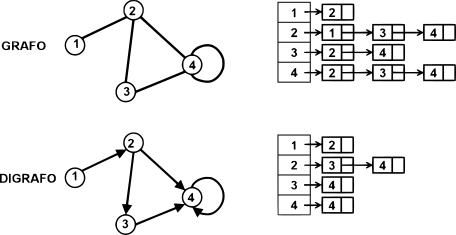
\includegraphics[scale=0.70]{Figuras/exemplos-grafo/r.png}
	\end{figure}
\end{frame}


\section{TAD Grafo}

\begin{frame}{TAD Grafo} 
	
	\justifying	
	
	\begin{itemize}
		\item Importante considerar os algoritmos em grafos como tipos abstratos de dados. 
		\item Conjunto de operações associado a uma estrutura de dados.
		\item Independência de implementação para as operações. 
		\item Devemos levar em conta o tipo de representação que iremos trabalhar
		\item Para nossa implementação iremos usar a representação por Lista de adjacência
		
	\end{itemize} 
\end{frame}

\begin{frame}{Implementação}
\lstinputlisting[language=C++]{Fontes/implementacao/impl-1.cpp}	
	
\end{frame}

\begin{frame}{Algumas operações sobre a TAD Grafo}
	\begin{enumerate}
		\item $IniciaGrafo(Grafo, N, Ponderado)$: Cria um grafo vazio. 
		\item $InsereAresta(Grafo, V1, V2, Peso)$: Insere uma aresta no grafo. 
		\item $ExisteAresta(Grafo, V1, V2)$: Verifica se existe uma determinada aresta.
		\item $ListaAdjacencia(Grafo, V)$: Obtém a lista de vértices adjacentes a um determinado vértice 
		\item $RetiraAresta(Grafo, V1, V2)$: Retira uma aresta do grafo.
		\item $ImprimeGrafo(Grafo)$: Imprime um grafo. 
		\item $LiberaGrafo(Grafo)$: Liberar o espaço ocupado por um grafo. 
		\item $GrauVertice(Grafo, V)$: Retorna o número de arestas incidentes (o número de vizinhos)
		\item $BuscaEmLargura(Grafo, VInical)$: Realiza uma Busca em Largura (BFS) a partir do vértice V
		\item $BuscaEmProfundidade(Grafo, VInicial)$: Realiza uma Busca em Profundidade (DFS)
		\item $MenorCaminho(Grafo, VInicial)$: Encontra o caminho de menor custo (Dijkstra)
	\end{enumerate}
		
		
\end{frame}

\begin{frame}{Implementação - Criando Grafo}
	\lstinputlisting[language=C++]{Fontes/implementacao/impl-2.cpp}	
	
\end{frame}


\begin{frame}{Implementação - Liberando o grafo}
	\lstinputlisting[language=C++]{Fontes/implementacao/impl-3.cpp}	
	
\end{frame}

\begin{frame}{Implementação - Inserindo aresta}
	\lstinputlisting[language=C++]{Fontes/implementacao/impl-4.cpp}	
	
\end{frame}

\begin{frame}{Implementação - Inserindo aresta}
	\lstinputlisting[language=C++]{Fontes/implementacao/impl-5.cpp}	
	
\end{frame}

\begin{frame}{Implementação - Retira Aresta}
	\lstinputlisting[language=C++]{Fontes/implementacao/impl-6.cpp}	
	
\end{frame}

\begin{frame}{Implementação - Imprime Aresta e Grau Vértice}
	\lstinputlisting[language=C++]{Fontes/implementacao/impl-7.cpp}	
	
\end{frame}


\begin{frame}{Teste Mesa}
	
	
	\begin{overlayarea}{\textwidth}{\textheight}
		\only<1>{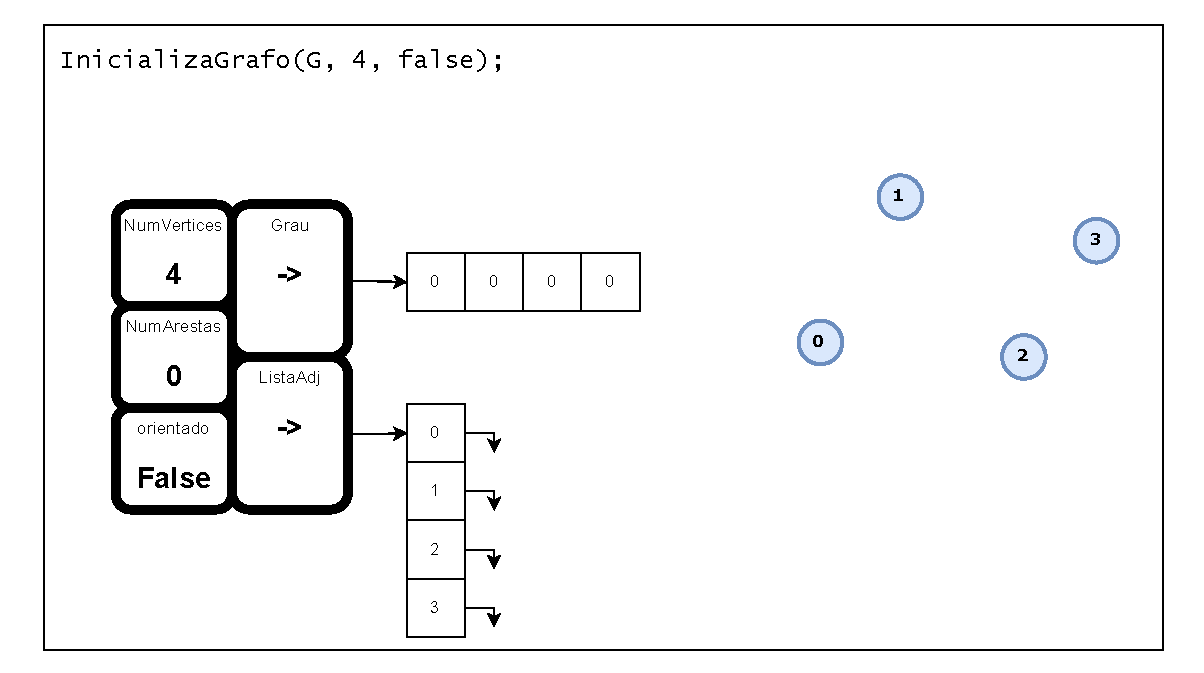
\includegraphics[scale=0.55]{Figuras/teste-mesa/mesa-1.pdf}}
		\only<2>{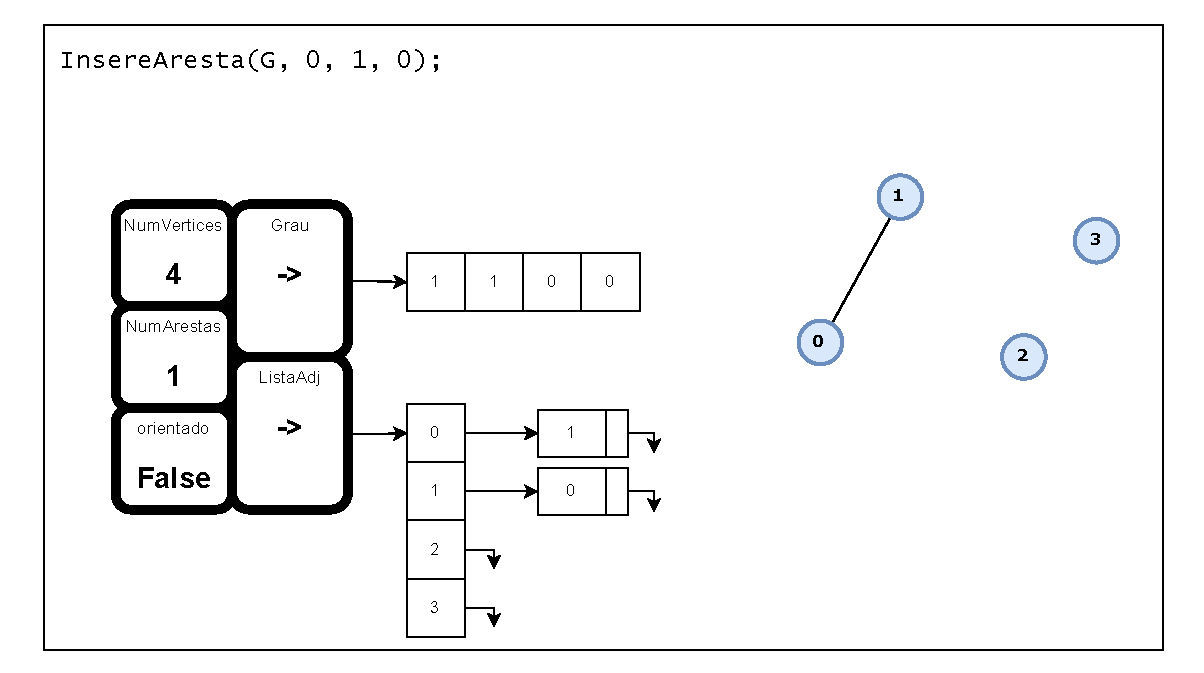
\includegraphics[scale=0.55]{Figuras/teste-mesa/mesa-2.pdf}}
		\only<3>{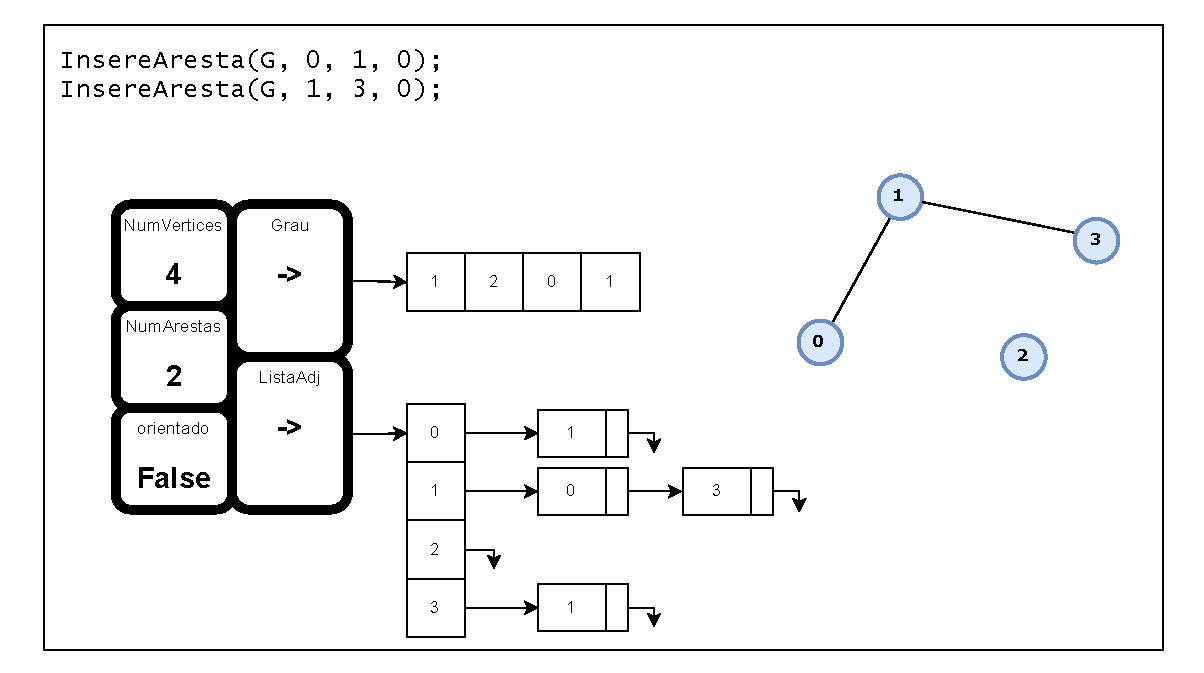
\includegraphics[scale=0.55]{Figuras/teste-mesa/mesa-3.pdf}}
		\only<4>{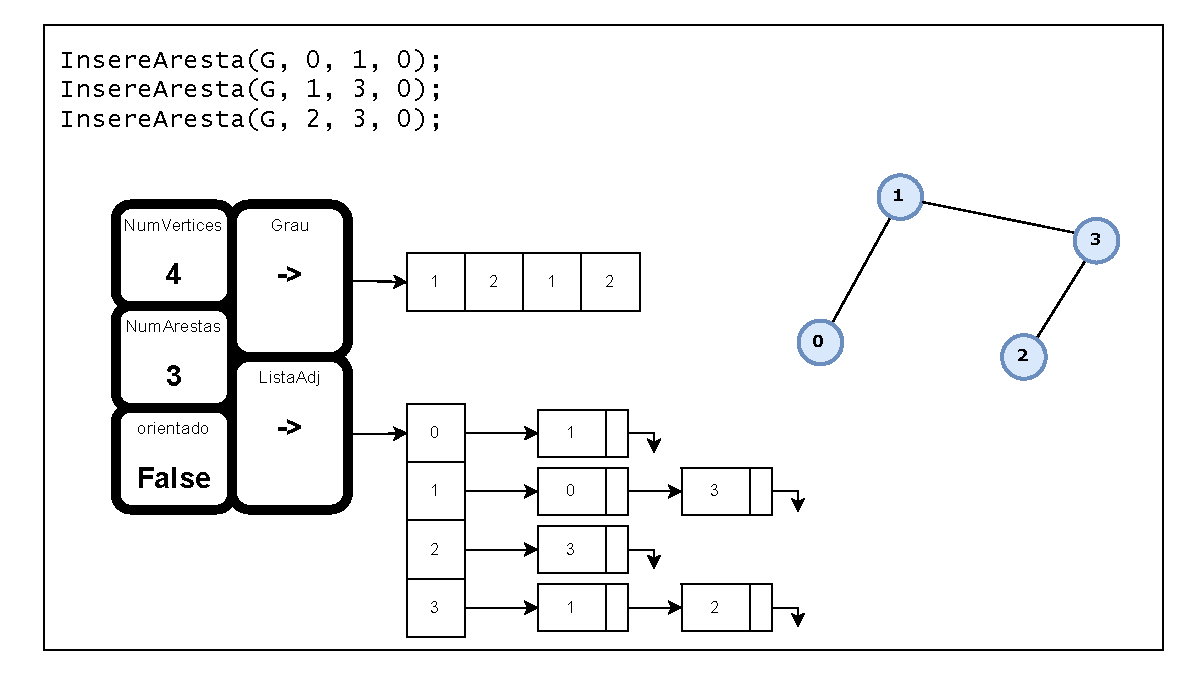
\includegraphics[scale=0.55]{Figuras/teste-mesa/mesa-4.pdf}}
		\only<5>{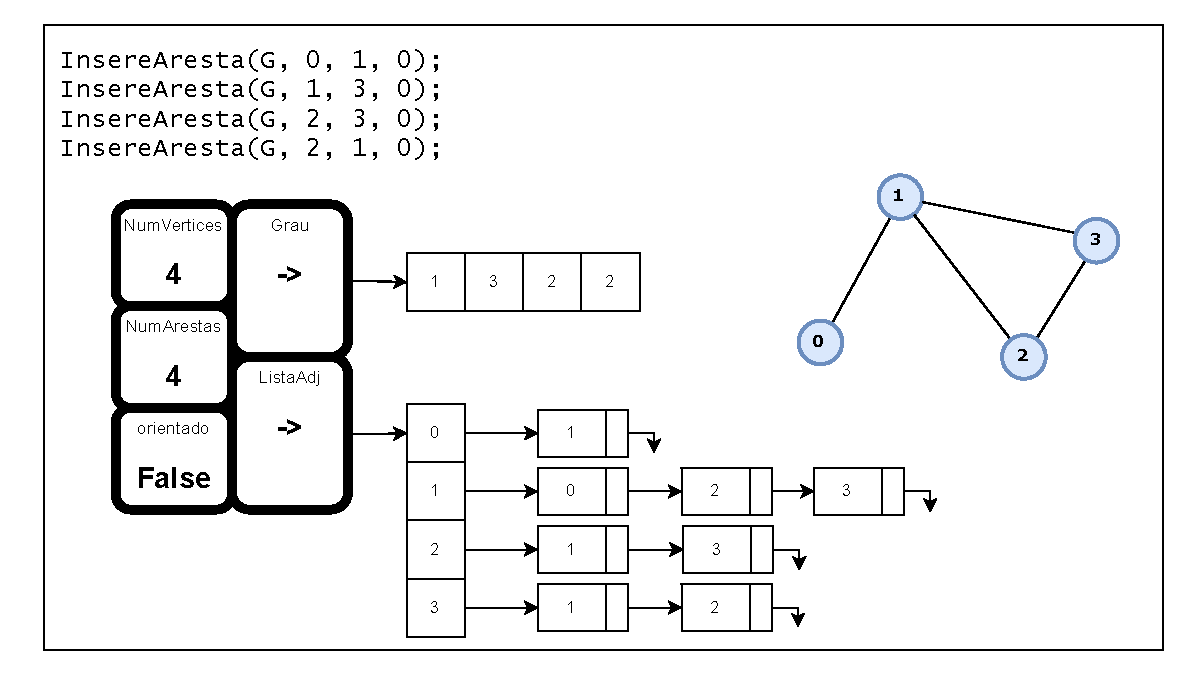
\includegraphics[scale=0.55]{Figuras/teste-mesa/mesa-5.pdf}}
		\only<6>{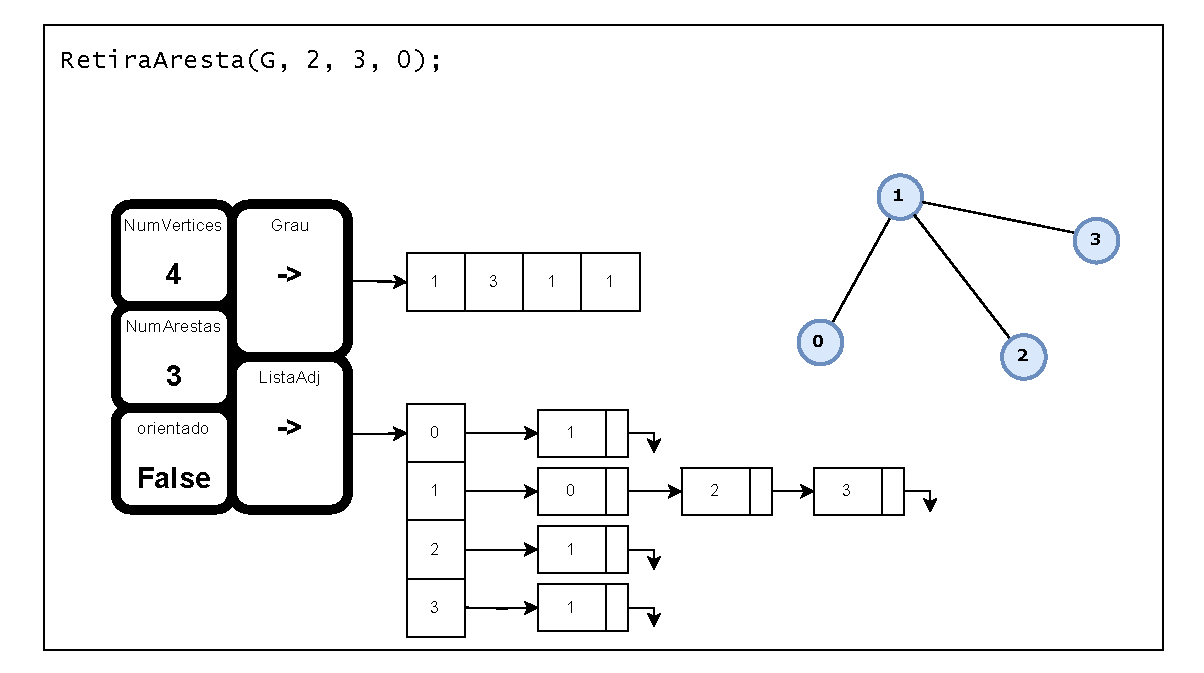
\includegraphics[scale=0.55]{Figuras/teste-mesa/mesa-6.pdf}}
		\only<7>{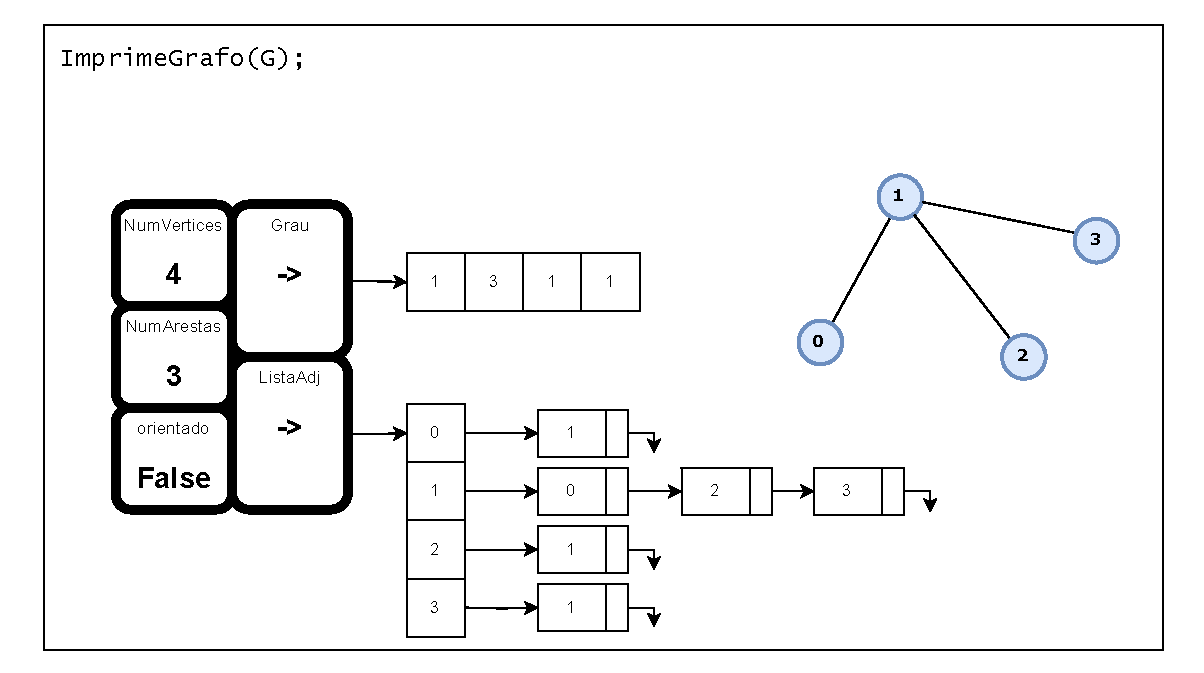
\includegraphics[scale=0.55]{Figuras/teste-mesa/mesa-7.pdf}}
		\only<8>{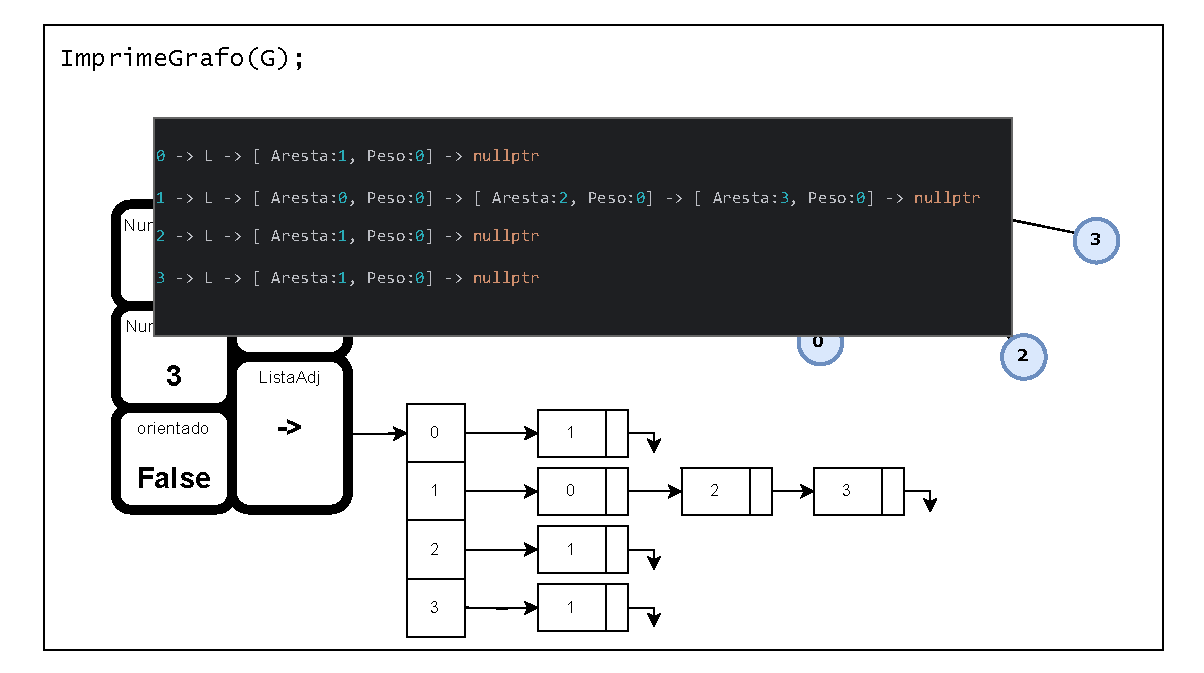
\includegraphics[scale=0.55]{Figuras/teste-mesa/mesa-8.pdf}}
		\only<9>{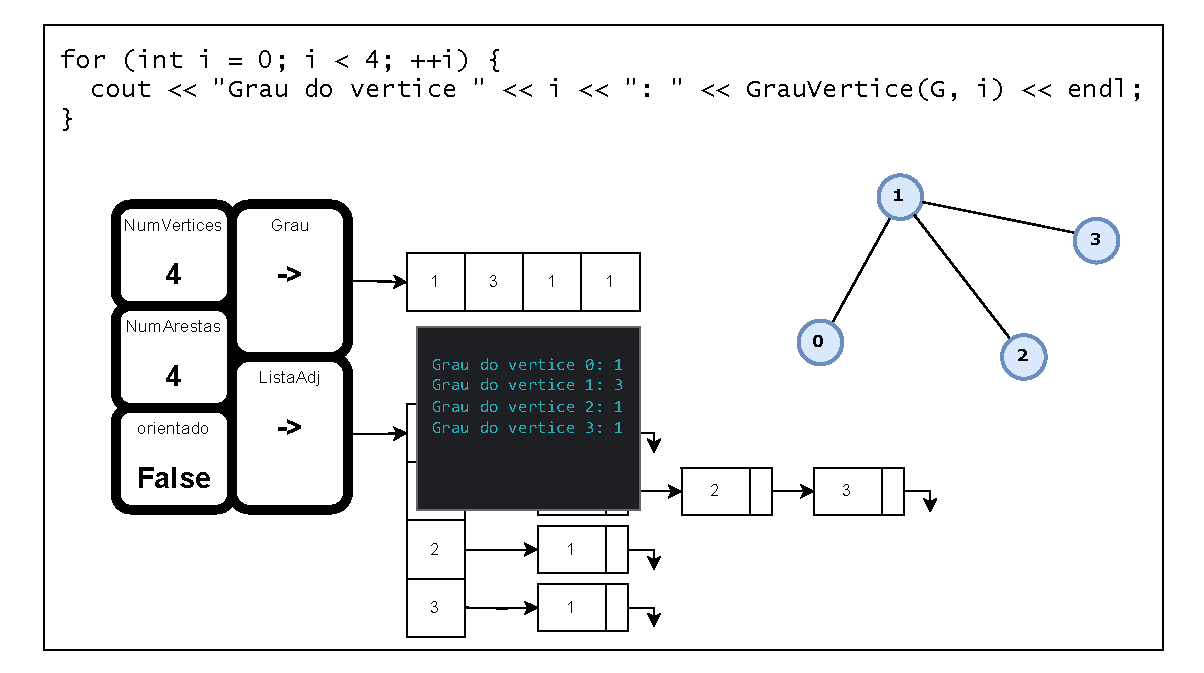
\includegraphics[scale=0.55]{Figuras/teste-mesa/mesa-9.pdf}}
		\only<10>{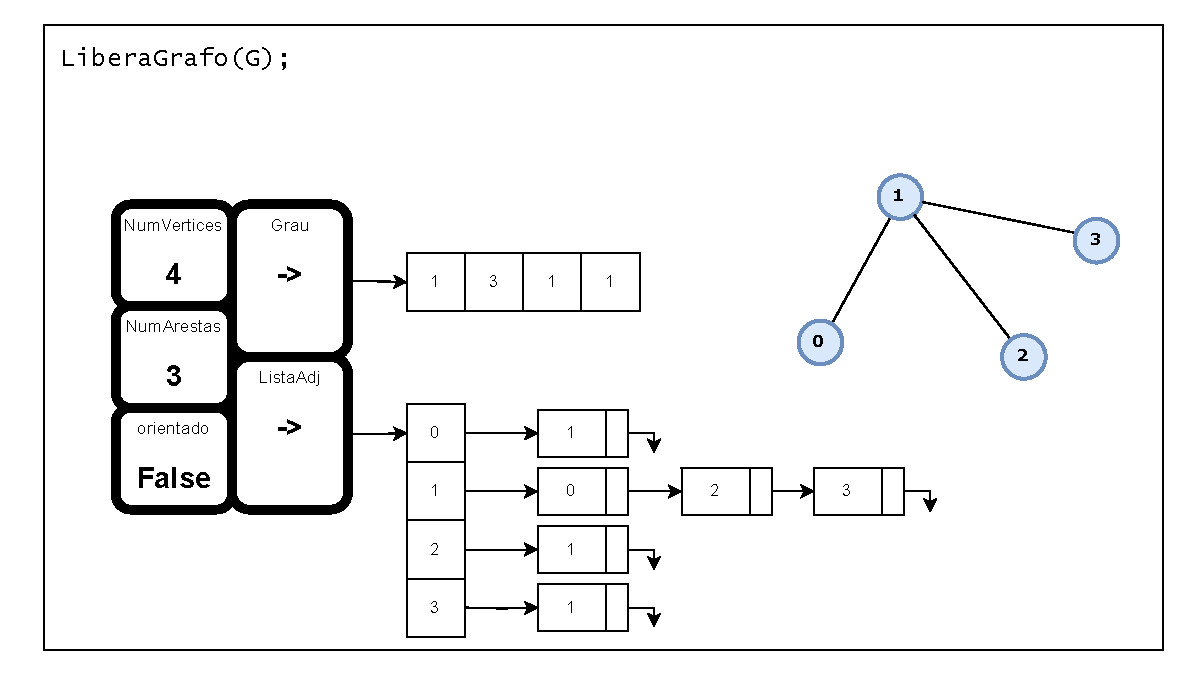
\includegraphics[scale=0.55]{Figuras/teste-mesa/mesa-10.pdf}}
		\only<11>{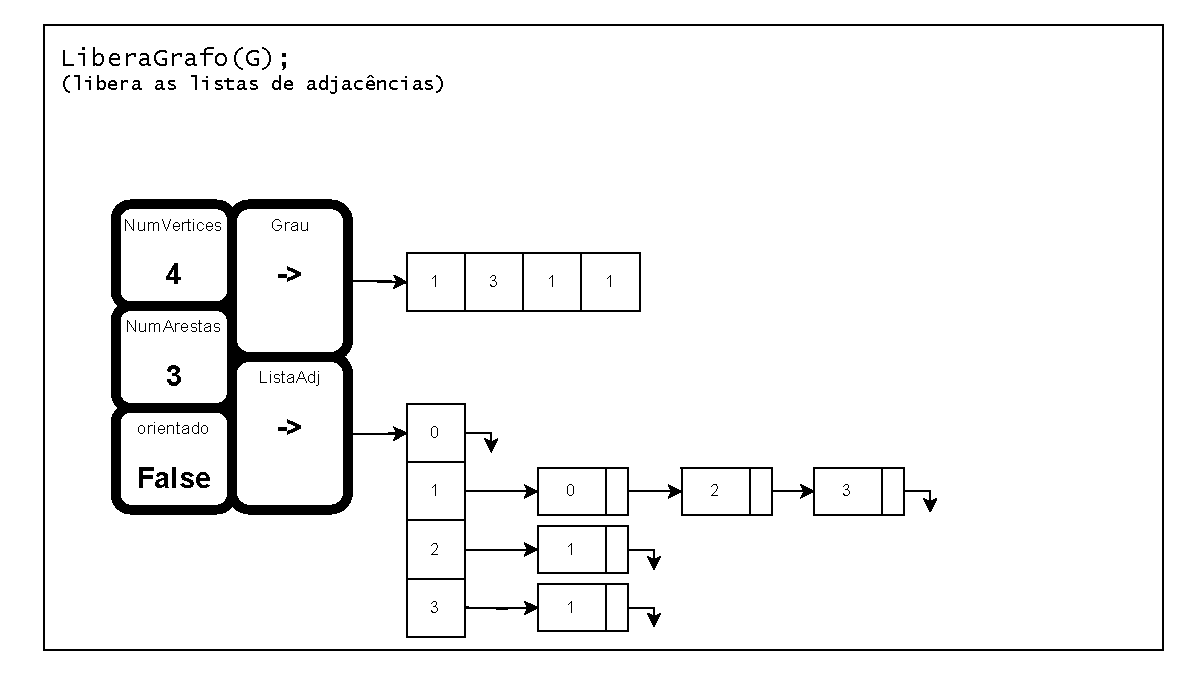
\includegraphics[scale=0.55]{Figuras/teste-mesa/mesa-11.pdf}}
		\only<12>{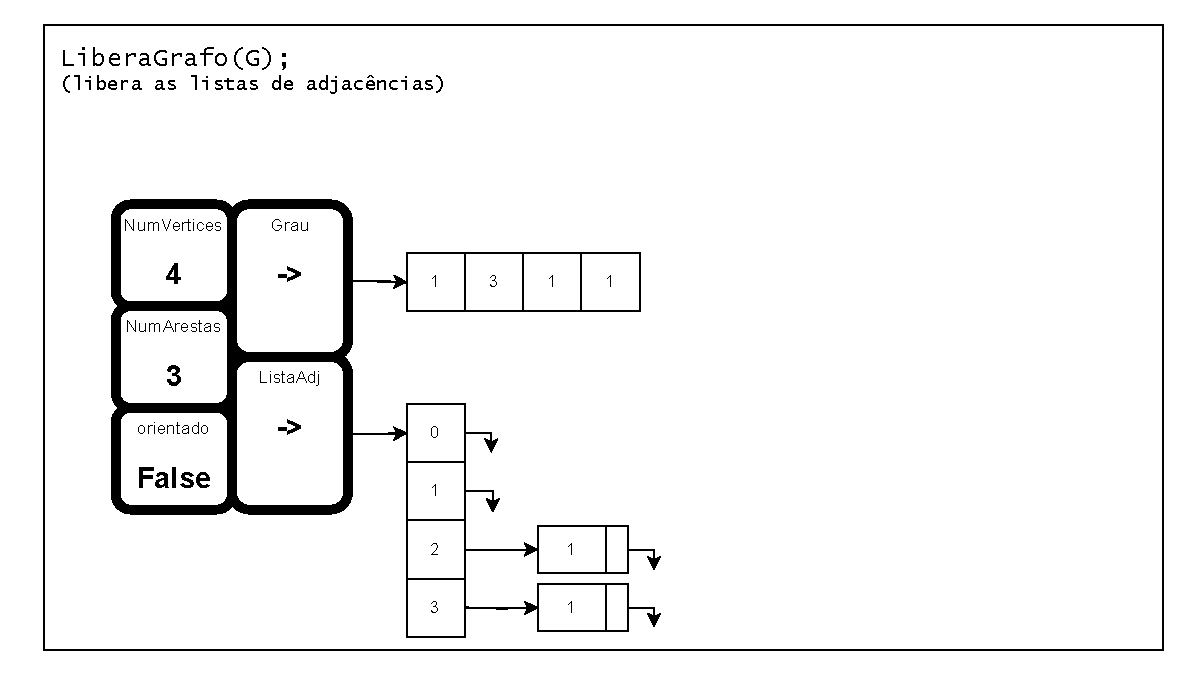
\includegraphics[scale=0.55]{Figuras/teste-mesa/mesa-12.pdf}}
		\only<13>{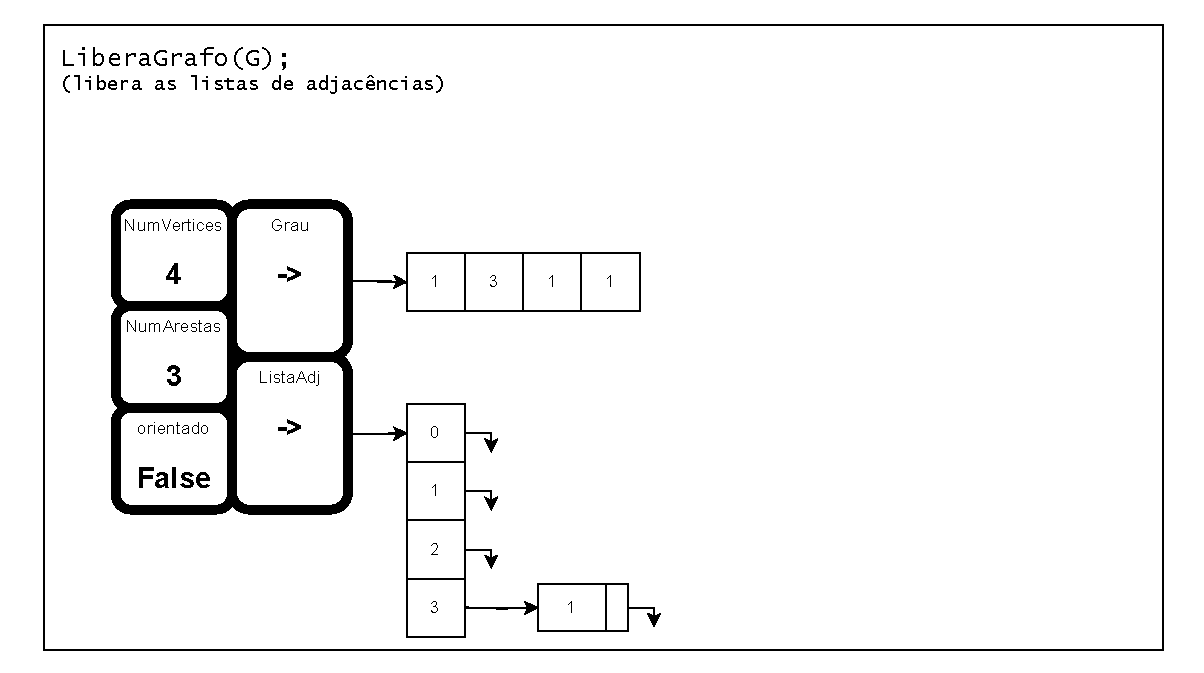
\includegraphics[scale=0.55]{Figuras/teste-mesa/mesa-13.pdf}}
		\only<14>{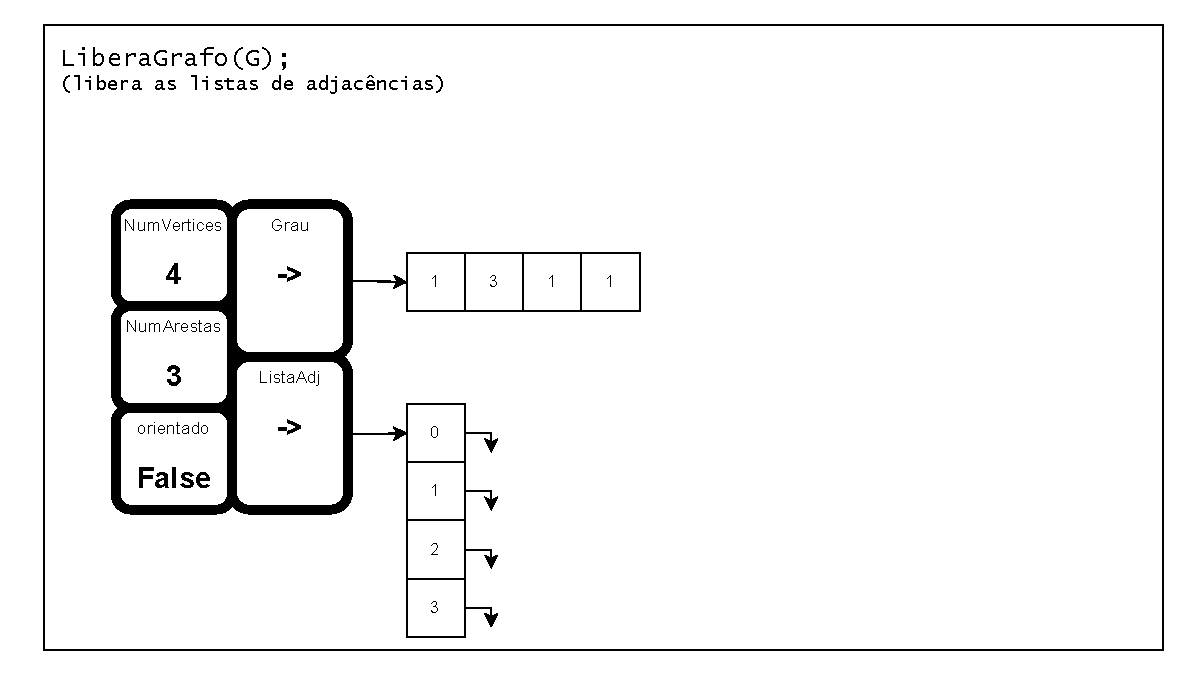
\includegraphics[scale=0.55]{Figuras/teste-mesa/mesa-14.pdf}}
		\only<15>{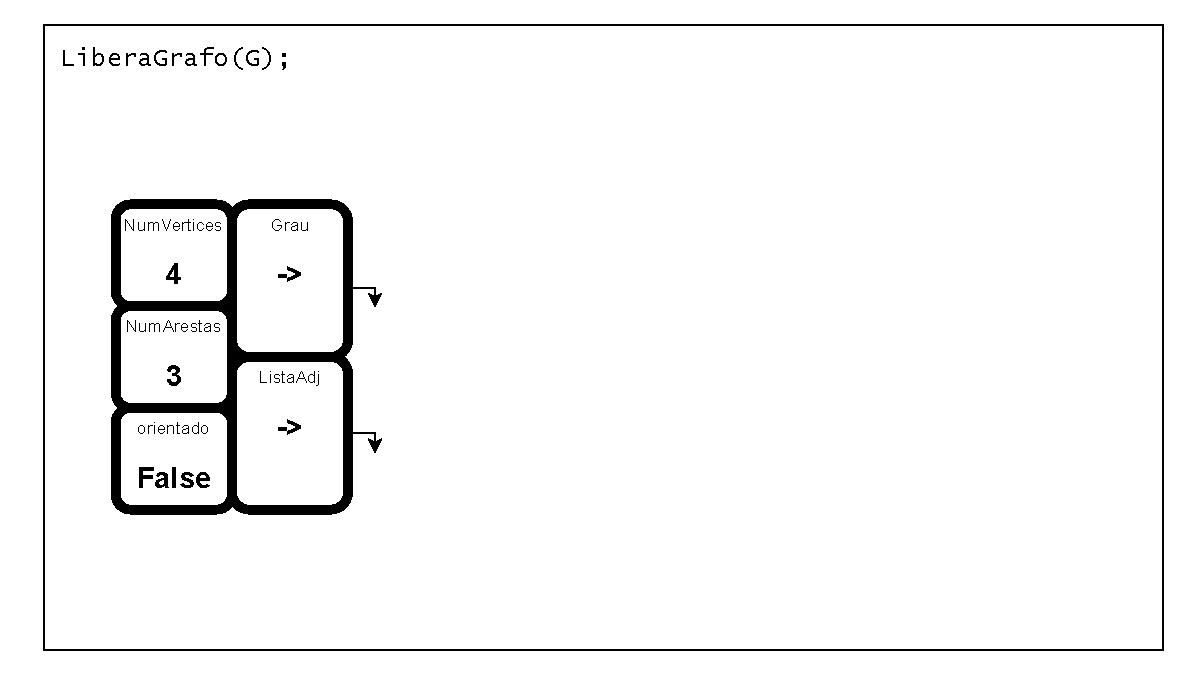
\includegraphics[scale=0.55]{Figuras/teste-mesa/mesa-15.pdf}}
		\only<16>{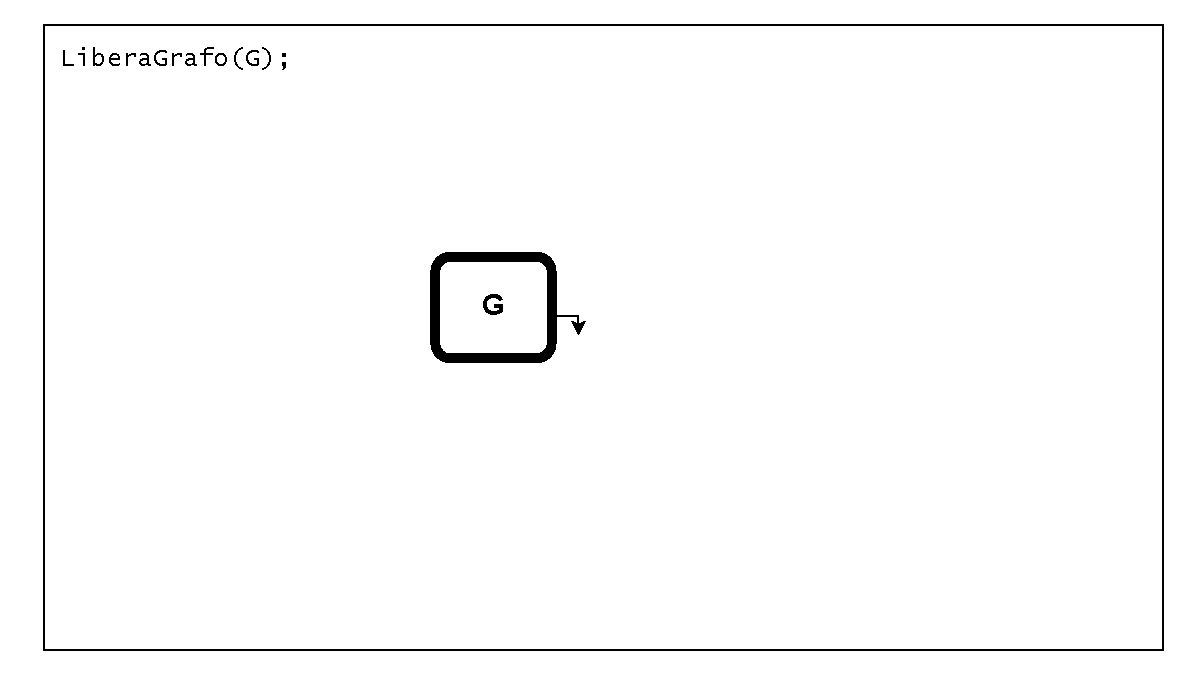
\includegraphics[scale=0.55]{Figuras/teste-mesa/mesa-16.pdf}}
	\end{overlayarea}
	
	
\end{frame}


\section{Busca em Grafos}

\begin{frame}{Busca em Grafos} 
	
	\justifying	
	\begin{overlayarea}{\textwidth}{\textheight}
		\only<1>{
			\begin{itemize}
				\item Consiste em explorar um grafo
				\item Buscas em grafos são processos algorítmicos que exploram sistematicamente os nós e arestas de um grafo.
				\item O objetivo é encontrar um caminho entre dois nós específicos, um nó específico ou todos os nós do grafo.
				\item Vários problemas em grafos podem ser resolvidos efetuando uma busca 
				\item A busca pode visitar todos ou apenas um subconjunto dos vértices.
			\end{itemize}
		}
		\only<2>{
			Existem vários tipos de algoritmos de busca que podemos realizar em um grafo. Os três principais:
			\begin{itemize}
				\item  Busca em largura
				\item  Busca em profundidade
				\item  Busca pelo menor caminho
			\end{itemize} 
		}
	\end{overlayarea}
\end{frame}


\begin{frame}{Busca em largura (BFS)} 
	
	\justifying
	
	\begin{itemize}
		\item Objetivo explorar um grafo de forma sistemática, visitando todos os nós em ordem crescente de distância do nó inicial.
		\item Partindo de um vértice inicial, a busca explora todos os vizinhos de um vértice. Em seguida, para cada vértice vizinho, ela repete esse processo, visitando os vértices ainda inexplorados.
		\item Pode ser usado para:
		\begin{enumerate}
			\item  Encontrar componentes conectados
			\item  Encontrar todos os vértices conectados a apenas um componente
			\item  Encontrar menor caminho entre dois vértices
			\item  Testar bipartição em grafos
		\end{enumerate}
	\end{itemize} 
\end{frame}


\begin{frame}{Busca em largura (BFS) - Algoritmo} 
	
	\justifying
	
	\begin{overlayarea}{\textwidth}{\textheight}
		\only<1>{
			\begin{itemize}
				\item Esse algoritmo faz uso do conceito de fila
				\item O grafo é percorrido de maneira sistemática, primeiro marcando como "visitados" todos os vizinhos de um vértice e em seguida começa a visitar os vizinhos de cada vértice na ordem em que eles foram marcados.
				\item Para realizar essa tarefa, uma fila é utilizada para administrar a visitação dos vértices.
			\end{itemize} 
			\lstinputlisting[language=pseudocodigo]{Fontes/implementacao/impl-8.txt}
		}
		\only<2>{
			\lstinputlisting[language=C++]{Fontes/implementacao/impl-9.cpp}	
		}
	\end{overlayarea}
	
		
\end{frame}


\begin{frame}{Teste Mesa}
	\justifying
	Considere o grafo G definido pelos arcos $0-2$, $0-3$, $0-4$, $1-2$, $1-4$, $2-4$, $3-4$, $3-5$, $4-5$, $5-1$
	
	\begin{overlayarea}{\textwidth}{\textheight}
		\only<1>{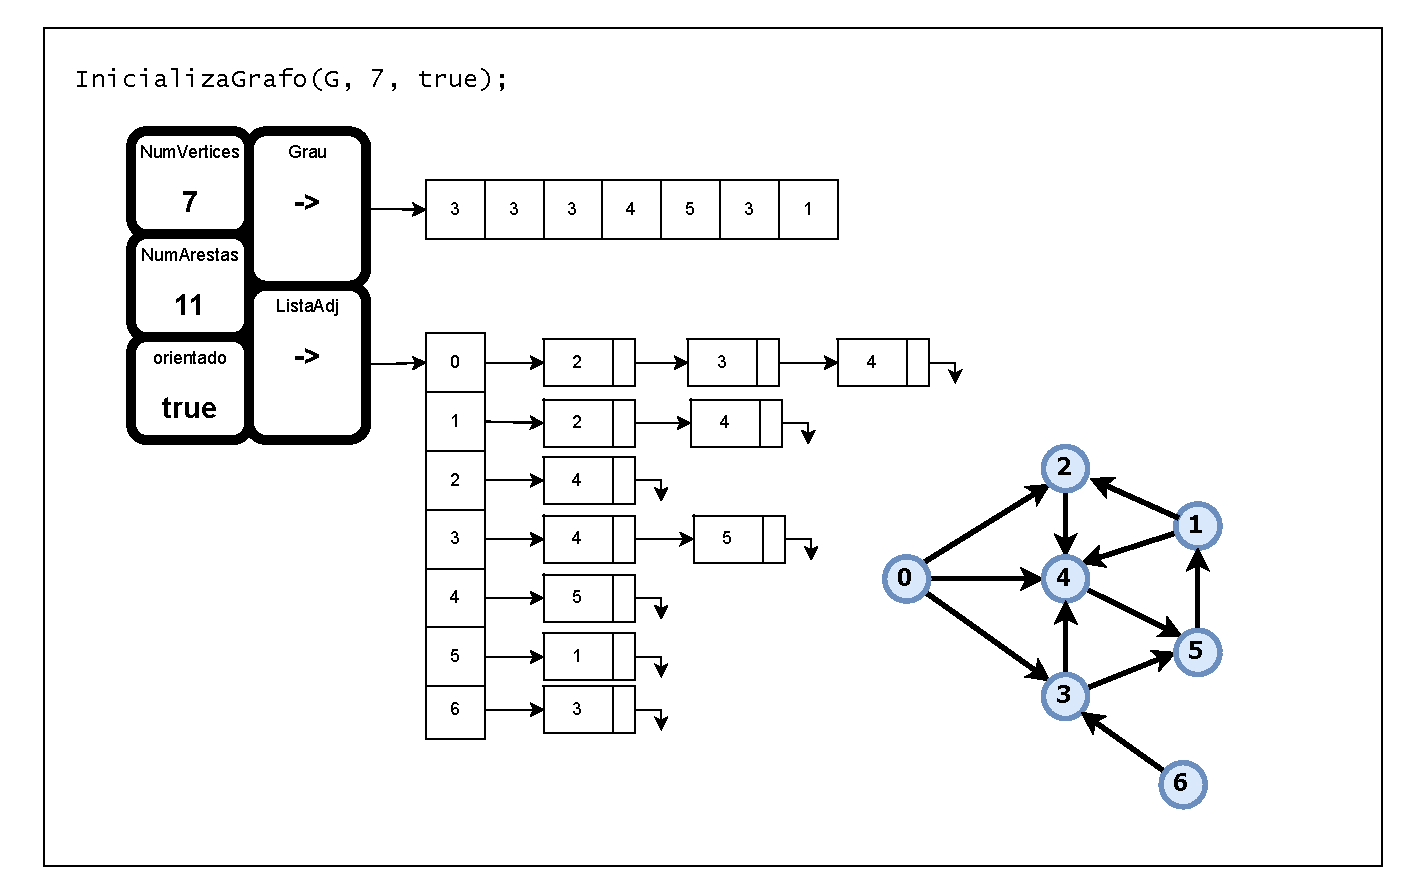
\includegraphics[scale=0.45]{Figuras/teste-mesa/mesa-17.pdf}}
		\only<2>{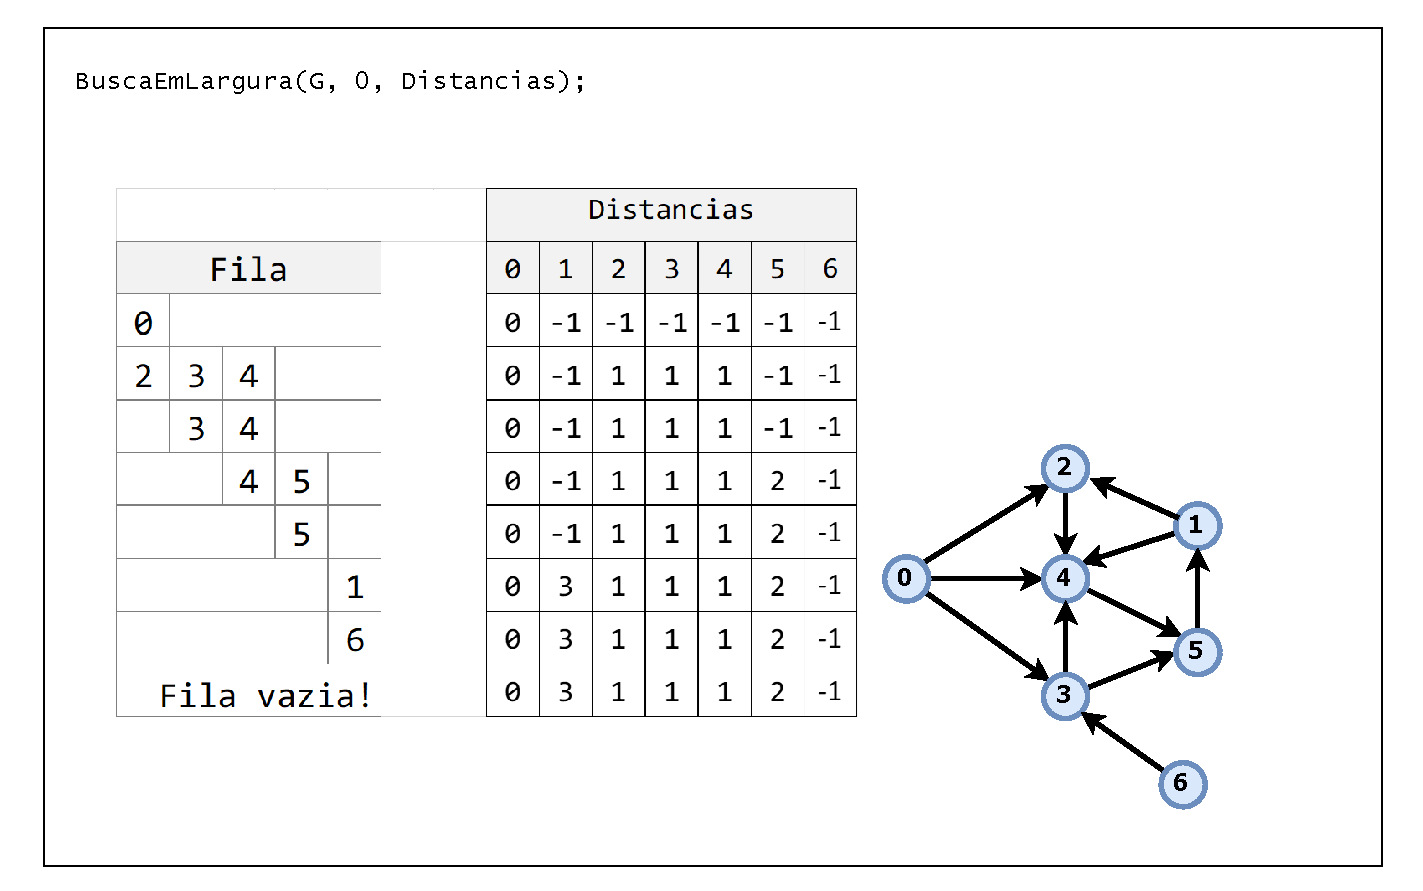
\includegraphics[scale=0.45]{Figuras/teste-mesa/mesa-18.pdf}}
	\end{overlayarea}
	
\end{frame}


\begin{frame}{Busca em profundidade DFS} 
	
	\justifying	

	\begin{itemize}
		\item Objetivo é visitar todos os vértices e numerá-los na ordem em que são descobertos.
		\item A busca em profundidade não resolve um problema específico.  Ela ajuda a compreender o grafo com que estamos lidando, revelando sua forma e reunindo informações (representadas pela numeração dos vértices) que ajudam a responder perguntas sobre o grafo. .
		\item Pode ser usado para:
		\begin{enumerate}
			\item  Encontrar componentes conectados e fortemente conectados;
			\item  Ordenação topológica de um grafo; 
			\item  Procurar a saída de um labirinto;
			\item  Verificar se um grafo é completamente conexo
		\end{enumerate}
	\end{itemize} 
\end{frame}


\begin{frame}{Busca em profundidade - Algoritmo} 
	
	\justifying	
	
	\begin{overlayarea}{\textwidth}{\textheight}
		\only<1>{
			\begin{itemize}
				\item Na busca em profundidade, as arestas são exploradas a partir do vértice inicial $v$ mais recentemente descoberto que ainda tem arestas não exploradas saindo dele.
				\item Quando todas as arestas de v são exploradas, a busca volta ao vértice anterior a v (backtracking) para seguir arestas ainda não exploradas.
				\item Ideia é identificar os caminhos a partir do vértice inicial.
			\end{itemize} 
		}
		\only<2>{
			Função BuscaEmProfundidade
			\begin{itemize}
				\item Esta função é a interface para a busca em profundidade.
				\item Recebe o grafo e o vértice inicial.
				\item Inicializa o vetor de distâncias com -1.
				\item o	Chama a função \textbf{BuscaEmProfundidadeRecursiva} para iniciar a busca a partir do vértice inicial.
			\end{itemize} 
			\lstinputlisting[language=C++]{Fontes/implementacao/impl-10.cpp}
		}
		\only<3>{
			Função BuscaEmProfundidadeRecursiva
			\begin{itemize}
				\item Esta função recursiva realiza a busca em profundidade.
				\item Ela recebe o grafo, o vértice atual, o vetor de distâncias e um contador para a distância.
				\item O vértice atual é marcado com a distância atual.
				\item A função itera sobre os vértices adjacentes ao vértice atual.
				\item Se um vértice adjacente ainda não foi visitado (distância -1), a função é chamada recursivamente para esse vértice.
			\end{itemize} 
			\lstinputlisting[language=C++]{Fontes/implementacao/impl-11.cpp}
		}
	\end{overlayarea}
	
			
\end{frame}

\begin{frame}{Teste Mesa}
	\justifying
	\begin{overlayarea}{\textwidth}{\textheight}
		\only<1>{
			Supondo essa implementação
			\lstinputlisting[language=C++]{Fontes/implementacao/impl-12.cpp}
			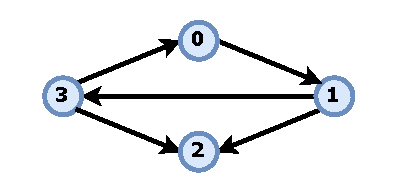
\includegraphics{Figuras/teste-mesa/mesa-19.pdf}
		}
		\only<2> {
			\textbf{Simulação da DFS:}
			\begin{enumerate}
				\item \textbf{Inicialização}: $Profundidades = [-1, -1, -1, -1]$, $cont = 0$, $VerticeInicial = 0$.
				\item \textbf{DFS(0)}:
					\begin{itemize}
						\item  $Profundidades[0] = 0$ (cont incrementado para 1)
						\item  Explora vértice 1 (adjacente a 0)
					\end{itemize}
				\item \textbf{DFS(1)}:
					\begin{itemize}
						\item  $Profundidades[1] = 1$ (cont incrementado para 2)
						\item  Explora vértice 2 (adjacente a 1)
					\end{itemize}  
				\item \textbf{DFS(2)}:
					\begin{itemize}
						\item  $Profundidades[2] = 2$ (cont incrementado para 3)
						\item  Sem vértices adjacentes não visitados. \textbf{Retorna para DFS(1)}
					\end{itemize}
				\item \textbf{DFS(1) continua}:
					\begin{itemize}
						\item  Explora vértice 3 (adjacente a 1)
					\end{itemize}
				\item \textbf{DFS(3)}:
					\begin{itemize}
						\item  $Profundidades[3] = 3$ (cont incrementado para 4)
						\item  Vértice 2 já foi visitado
						\item  Vértice 0 já foi visitado. Retorna para DFS(1
					\end{itemize}
				\item \textbf{DFS(1) continua}: Todos os vértices adjacentes a 1 foram explorados. Retorna para DFS(0).
				\item \textbf{DFS(0) continua}: Todos os vértices adjacentes a 0 foram explorados. Finaliza a DFS.
				
					
			\end{enumerate}
		}
		\only<3> {
			\textbf{Resultado e analise do vetor de profundidade}: $ Profundidades = [0, 1, 3, 2] $
			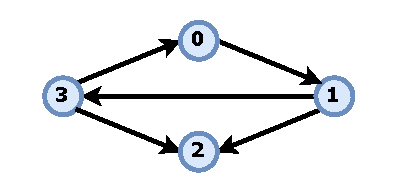
\includegraphics{Figuras/teste-mesa/mesa-19.pdf}
			\begin{itemize}
				\item Ordem de Exploração
				\begin{enumerate}
					\item  O vértice $0$ foi visitado primeiro ($Profundidade[0] = 0$)
					\item  O vértice $1$ foi visitado em segundo ($Profundidade[1] = 1$)
					\item  O vértice $3$ foi visitado em terceiro ($Profundidade[3] = 2$)
					\item  O vértice $2$ foi visitado por último ($Profundidade[2] = 3$)
				\end{enumerate}
				\item para uma análise mais completa é necessário, que durante a execução da DFS, registrar outros dados auxiliares como o pai de cada vértice na árvore.
			\end{itemize}
		}
	\end{overlayarea}
	
	
	
\end{frame}



\begin{frame}{Busca pelo menor caminho} 
	
	\justifying	
	
	\begin{overlayarea}{\textwidth}{\textheight}
		\only<1>{
			\begin{itemize}
				\item Partindo de um vértice inicial, calcula a menor distância desse vértice a todos os demais (Desde que exista um caminho entre eles)
				\item O comprimento pode ser o número de arestas que conectam os dois vértices ou a soma dos pesos das arestas que compõem esse caminho (grafo ponderado)
				\item Uma das maneiras de achar o menor caminho é utilizando o algoritmo de Dijkstra (um dos algoritmos mais conhecido)
			\end{itemize} 
		}
		\only<2>{
			{\bfseries Apresentando Dijkstra }% do not use \bf in LaTeX it is deprecated 20+ years ago
			
			\begin{minipage}{.55\textwidth}
				\begin{itemize}% never number things manually!
					\item Nome: Edsger Wybe Dijkstra
					\item Criação do algoritmo: 1956
					\item Importância: Um dos algoritmos mais importantes da ciência da computação, usado em diversas aplicações.
					\item Trabalha com grafos e digrafos, ponderados ou não. No caso de um grafo ponderado, as arestas não podem ter pesos negativos
				\end{itemize}
			\end{minipage}
			\hfill
			\begin{minipage}{.35\textwidth}
				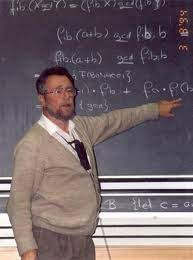
\includegraphics[scale=0.6]{Figuras/dijkstra.jpg}
			\end{minipage}
		}
	\end{overlayarea}
	
	
\end{frame}

\begin{frame}{Passos do Algoritmo} 
	
	\justifying	
	
	\begin{overlayarea}{\textwidth}{\textheight}
		\only<1>{
			\begin{enumerate}
				\item \textbf{Inicialização:}
				\begin{itemize}
					\item Atribua a distância do vértice de origem para ele mesmo como 0.
					\item Atribua a distância de todos os outros vértices como infinito, pois ainda não sabemos a distância real.
					\item Defina o vértice predecessor de todos os vértices como indefinido, pois ainda não sabemos por qual vértice chegamos a cada um.
				\end{itemize}
				\item Comece no vértice de origem.
				\item Explore os vértices adjacentes (vizinhos) e calcule a distância até eles.
				\item Marque o vértice com a menor distância como "visitado".
				\item Repita os passos 2 e 3 a partir do vértice visitado, explorando novos vizinhos.
				\item Continue até alcançar o vértice de destino.
			\end{enumerate}
			
		}
		\only<2>{
			\lstinputlisting[language=C++]{Fontes/implementacao/impl-13.cpp}
		}
		\only<3>{
			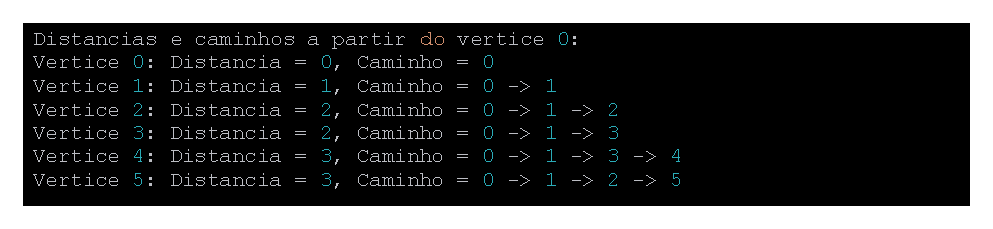
\includegraphics[scale=0.70]{Figuras/teste-mesa/mesa-20.pdf}
			\centering
			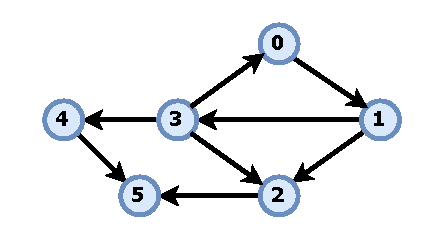
\includegraphics[scale=0.8]{Figuras/teste-mesa/mesa-21.pdf}
		}
	\end{overlayarea}
	
	
\end{frame}


\section{Exemplo Prático com Neo4j}

\begin{frame}{Exemplo Prático com Neo4j} 
	
	O Neo4j é um banco de dados NoSQL (orientado a grafo) de código aberto que se destaca por sua capacidade de armazenar e consultar dados como um grafo, em vez de tabelas como nos bancos de dados relacionais.
	
	\emph{Modelo de Dados em Grafos}
	\vspace{0.3cm}
	\begin{itemize}
		\item \textbf{Nós (Nodes)}: Representação de entidades (vértices).
		\item \textbf{Relacionamentos (Relationships)}: Conexões entre nós (arestas).
		\item \textbf{Propriedades (Properties)}: Atributos que podem ser associados a nós e relacionamentos.
	\end{itemize}
	
\end{frame}

\begin{frame}{Cypher} 
	\begin{overlayarea}{\textwidth}{\textheight}
		\only<1>{
			Cypher é a linguagem de consulta declarativa de Neo4j e utiliza uma sintaxe inspirada em ASCII-art.
			
			\par{Elementos da Linguagem}
			
			\begin{enumerate}
				\item \textbf{Nós}: Representados por parênteses \texttt{()}, os nós podem ter propriedades no formato chave:valor. Exemplo:
				\lstinputlisting[language=Cypher,firstline=1,lastline=1]{Fontes/implementacao/impl-14.txt}
				
				\item \textbf{Relacionamentos}: Representados por setas \texttt{-->} ou \texttt{<--} para indicar a direção, os relacionamentos conectam dois nós e também podem ter propriedades. Exemplo:
				\lstinputlisting[language=Cypher,firstline=2,lastline=2]{Fontes/implementacao/impl-14.txt}
				
				\item \textbf{Cláusulas}: As cláusulas adicionam lógica às nossas consultas:
				\begin{itemize}
					\item \textbf{MATCH}: Encontra padrões no grafo.
					\item \textbf{WHERE}: Filtra resultados com base em condições.
					\item \textbf{RETURN}: Define os dados que queremos retornar.
					\item \textbf{CREATE}: Cria novos nós e relacionamentos.
					\item \textbf{SET}: Atualiza propriedades de nós e relacionamentos.
					\item \textbf{DELETE}: Remove nós e relacionamentos.
				\end{itemize}
			\end{enumerate}
		}
		\only<2>{
			\emph{Exemplos de Consultas em Cypher}
			\begin{enumerate}
				\item Criação de Nós e Relacionamentos:
				\lstinputlisting[language=Cypher,firstline=3,lastline=5]{Fontes/implementacao/impl-14.txt}
				
				\item Consulta de Nós e Relacionamentos:
				\lstinputlisting[language=Cypher,firstline=6,lastline=7]{Fontes/implementacao/impl-14.txt}
				
				\item Atualização de Dados:
				\lstinputlisting[language=Cypher,firstline=8,lastline=9]{Fontes/implementacao/impl-14.txt}
				
				\item Exclusão de Nós e Relacionamentos:
				\lstinputlisting[language=Cypher,firstline=10,lastline=11]{Fontes/implementacao/impl-14.txt}
				
				\item Consulta com cláusula WHERE:
				\lstinputlisting[language=Cypher,firstline=12,lastline=14]{Fontes/implementacao/impl-14.txt}
			\end{enumerate}
			
		}
	\end{overlayarea}
	
\end{frame}

\begin{frame}{Hands on} 
	\begin{overlayarea}{\textwidth}{\textheight}
		\only<1>{
	
			Para ficar mais visível a aplicabilidade do neo4j, vamos discutir uma solução de uma rede social simples com onde o modelo de dados é baseado em grafos
			
			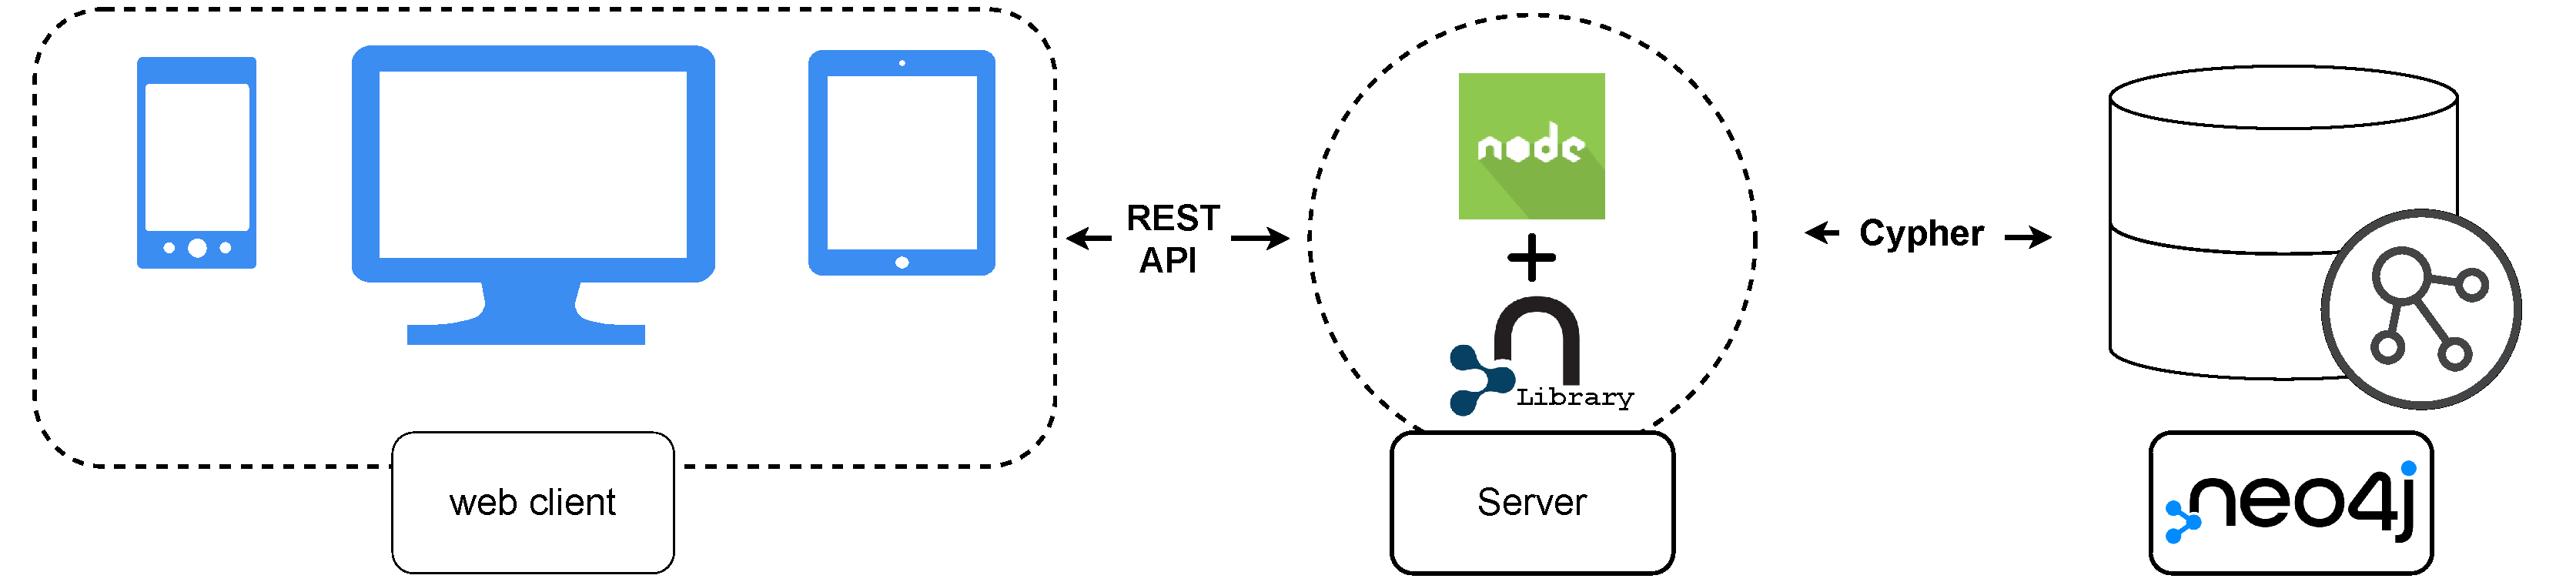
\includegraphics[scale=0.20]{Figuras/arq.pdf}
			
			No caso foi uma solução de rede social simples utilizando Angular para o frontend, nodeJs para backend e Neo4j como banco de dados
			
			\emph{Funcionalidades}
			\begin{enumerate}
				\item \textbf{Login Simples:} Usuários fazem login utilizando apenas o número de matrícula.
				
				\item \textbf{Feed de Postagens:} Todos os usuários podem fazer publicações e visualizar as postagens de todos.
				
				\item \textbf{Curtidas em Postagens:} Usuários podem curtir postagens.
			\end{enumerate}	
		}
		\only<2> {
			\emph{Modelagem no Neo4j}\par
			Visão detalhada da modelagem dos dados no Neo4j para nossa aplicação:
			\begin{enumerate}
				\item Nodos (Nodes):
				\begin{itemize}
					\item \textbf{Usuário (User):} Representa cada usuário da rede social. 
					\begin{itemize}
						\item Propriedades: nome, matrícula.
					\end{itemize}
					\item \textbf{Postagem (Post):} Representa cada postagem no feed.
					\begin{itemize}
						\item Propriedades: content (conteúdo da postagem), timestamp (data e hora da postagem), id (identificador único).
					\end{itemize}
				\end{itemize}
				\item Relações (Relationships):
				\begin{itemize}
					\item \textbf{POSTADO:} Conecta um usuário a uma postagem que ele criou. 
					\begin{itemize}
						\item Indica que um determinado usuário fez uma determinada postagem.
					\end{itemize}
					\item \textbf{CURTE (LIKES):} Conecta um usuário a uma postagem que ele curtiu. 
					\begin{itemize}
						\item Permite calcular o número de curtidas de cada postagem.
					\end{itemize}
				\end{itemize}
			\end{enumerate}
		}
		\only<3> {
			\emph{Comandos Cypher utilizados no nosso sistema}\par
			\begin{enumerate}
				\item Criação dos Usuários:
				\lstinputlisting[language=Cypher,firstline=15,lastline=15]{Fontes/implementacao/impl-14.txt}
				
				\item Login(consulta usuário):
				\lstinputlisting[language=Cypher,firstline=16,lastline=16]{Fontes/implementacao/impl-14.txt}
				
				\item Criar uma Postagem:
				\lstinputlisting[language=Cypher,firstline=17,lastline=18]{Fontes/implementacao/impl-14.txt}
				
				\item Obter Todas as Postagens:
				\lstinputlisting[language=Cypher,firstline=24,lastline=27]{Fontes/implementacao/impl-14.txt}
				
				\item Curtir uma Postagem:
				\lstinputlisting[language=Cypher,firstline=28,lastline=29]{Fontes/implementacao/impl-14.txt}
			\end{enumerate}
		}
	\end{overlayarea}
	
\end{frame}

\begin{frame}{Hora de experimentar!}
	
	\begin{minipage}{.75\textwidth}
		No grafo já foi cadastrado os nodes users:	
		\begin{itemize}% never number things manually!
			\item Todos os alunos da nossa matéria
			\item E o professor - 0001
		\end{itemize}
		A demonstração está disponível aqui: \url{ https://demo-grafos.carlos-henreis.com.br/}\par
		Acesso é com número de matricula (o do professor é especial 0001)
	\end{minipage}
	\hfill
	\begin{minipage}{.25\textwidth}
		
\includegraphics[scale=0.03]{Figuras/qr-code.pdf}
	\end{minipage}

\end{frame}


\section{Referências} 

\begin{frame}{Referências}
	
	\begin{enumerate}
		\item Backes, A. (2017). \textit{Estrutura de Dados Descomplicada-em Linguagem C}. Elsevier Brasil.
		
		\item Feofiloff, P. \textit{Algoritmos para Grafos}, \\ \texttt{http://www.ime.usp.br/~pf/algoritmos\_para\_grafos/} \\ (última visita 17/05/2024)
		
		\item LAL, Mahesh. \textit{Neo4j graph data modeling}. Packt Publishing Ltd, 2015.
		
		\item ZIVIANI, Nivio et al. \textit{Projeto de algoritmos: com implementações em Pascal e C}. Cengage, 2011.
	\end{enumerate}

\end{frame}

%\begin{frame}
%\begin{figure}
%\centering
%\includegraphics[scale=0.3]{oraculo.jpg}
%\caption{Questões importantes!}
%\end{figure}
%\end{frame}

\end{document}
